\documentclass{beamer}
\usetheme[deutsch]{KIT}

\KITfoot{Tutoriumsmaterial von Simon Stroh und Moritz v. Looz}
\usepackage[utf8]{inputenc}
\usepackage{amsmath}
\usepackage{ulem}
\usepackage{ifthen}
\usepackage{amssymb}
\usepackage{tikz}
\usetikzlibrary{automata}
\usenavigationsymbols


\title{Theoretische Grundlagen der Informatik}
\subtitle{Tutorium}
\author{Moritz von Looz, Simon Stroh}

\institute[ITI]{Intitute für Theoretische Informatik}

\TitleImage[height=\titleimageht]{images/tmaschine.png}

\begin{document}
\begin{frame}
  \maketitle
\end{frame}

%%%%%%%%%%%%%%%%%%%
% Switch to render everything or only newest part.
\ifthenelse{1=1}{}{
%%%%%%%%%%%%%%%%%%%


\section{Organisatorisches}
\begin{frame}
	\frametitle{Organisatorisches - Zum Übungsbetrieb}
	\begin{itemize}
		\item \textbf{Abgabe:} \emph{Handschriftlich} in Zweiergruppen.
		\item \textbf{Schein:} 
		\begin{itemize}
			\item Klausurbonus
			\item Wahrscheinlich ein Notenschritt
			\item Ab 50\% der erreichbaren Punkte
		\end{itemize}
		\item Tutoriumsmaterial und Aktueller Punktestand online.
		\begin{itemize}
			\item URL wird noch bekanntgegeben
			\item Wer Punkte online einsehen will, email in Liste eintragen
		\end{itemize}
	\end{itemize}
\end{frame}
\begin{frame}
	\frametitle{Organisatorisches - Zum Tutorium}
	\begin{itemize}
		\item Stoff soll wiederholt werdet
		\item Dabei Fokus auf Übungsbetrieb
		\item Fragen/Vorschläge/Anmerkungen wilkommen!
		%\item Wer Tee möchte darf sich bedienen :)
	\end{itemize}
\end{frame}
\section{Endliche Automaten und reguläre Sprachen}
\subsection{Formale Sprachen}
\begin{frame}
	\frametitle{Kurze Wiederholung: Formale Sprachen}
	Eine \emph{Formale Sprache} $L$ ist eine Teilmenge aller Wörtern über einem endlichen Alphabet $\Sigma$. Also $L \subseteq \Sigma^*$\\[0.3cm]
	Beispiele:
	\KITframe[yes the background would be nice in gray, thanks!]
		{\parbox{\textwidth}{\begin{itemize}
			\item $\Sigma = \{ 0, 1 \}, L = \{w11z\,|\,w,z \in \Sigma^*\}$
			\begin{itemize}
			\item Die Menge aller Wörter die ''11'' enthalten.
			\end{itemize}
		\end{itemize}}
	}\\[0.2cm]
Im Allgemeinen kann man Formale Sprachen sehr frei angeben: 
	\KITframe[Yeah, I think I'll stick to gray as a background color. Thanks again!]
		{\parbox{\textwidth}{\begin{itemize}
			\item $\Sigma = \{ 0, 1 \}, L = \{w|\,w \in \Sigma^*, w \mbox{ hat eine gerade Anzahl an $1$en}\}$
			\begin{itemize}
			\item Die Menge aller Wörter die eine gerade Anzahl an Einsen enthalten.
			\end{itemize}
		\end{itemize}}
	}
\end{frame}
\subsection{Reguläre Sprachen}
\begin{frame}
 \frametitle{Wiederholung der Wiederholung: Reguläre Sprachen}
        Eine Sprache \(L\subseteq\Sigma^*\) heißt regulär, wenn für sie eine der folgenden Punkte gilt:

\begin{itemize}
\item \begin{itemize}Verankerung
\item \(L = {a}\) mit \(a\in\Sigma^*\) oder
\item \(L = \varnothing \)
\end{itemize}
\item \begin{itemize}Induktion: Seien \(L_1\), \(L_2\) reguläre Sprachen
      \item \(L = L_1 \cdot L_2\) oder
      \item \(L = L_1 \cup L_2\) oder
      \item \(L = L_1^*\)
      \end{itemize}

\end{itemize}
Beispiel:
\(\Sigma = \{a,b\}\)
	\KITframe[Yeah, I think I'll stick to gray as a background color. Thanks again!]
		{\parbox{\textwidth}{\begin{itemize}
		\item \(L_1 = \{w| w \in \Sigma^*, w \mbox{w besteht aus einer graden Anzahl $a$s}\)
		\item \(L_2 =\{w| w \in \Sigma^*, w \mbox{w enthält gleich viele $a$s und $b$s.}\)		
		\end{itemize}}
	}
	\(L_1\) ist regulär, \(L_2\) nicht.
\end{frame}

\subsection{Deterministische endliche Automaten}
\begin{frame}
\frametitle{Deterministische Endliche Automaten}
        Ein deterministischer endlicher Automat $M$ ist ein 5-Tupel
        \[
        M= (Q,\Sigma,\delta,S,F).
        \]
        \begin{itemize}
        \item $Q$:  endliche Zustandsmenge
        \item $\Sigma$:    endliches Alphabet
        \item $\delta$:   Zustandsübergangsfunktion $Q\times \Sigma \rightarrow Q$
        \item $S$:   Startzustand $\in Q$
        \item $F$:   Endzustandsmenge $\subseteq Q$
        \end{itemize}
\end{frame}
\begin{frame}
	\frametitle{DEA: Aufgaben}
	\begin{enumerate}
	\item 
		Lösen Sie folgendes Rätsel mit Hilfe eines deterministischen
		endlichen Automaten:
		\begin{quote}
		  Es stehen drei Wasserkrüge mit einem Fassungsvermögen
		  von 3, 5 bzw. 7 $l$ zur Verfügung, um eine Wassermenge von
		  einem Liter abzumessen, d.~h. in einem der Krüge soll sich genau
		  diese Menge Wassers befinden. Zu Beginn sind der kleinste und
		  der größte Krug gefüllt. Da Ihr Augenmaß schlecht
		  ist, darf Wasser nur so von einem Krug in einen anderen
		  gegossen werden, dass der eine ganz geleert oder der andere
		  ganz gefüllt wird (ohne dass Wasser verschüttet wird).
		\end{quote}
		Geben Sie den Übergangsgraphen eines Automaten an, dessen
		akzeptierte Sprache genau die zulässigen lösenden
		Umfüllreihenfolgen kodiert, sowie ein kürzestes Lösungswort.
	\end{enumerate}
\end{frame}
\begin{frame}
\frametitle{DEA: Aufgabe}
\begin{enumerate}
\setcounter{enumi}{1}
\item Geben Sie einen regulären Ausdruck für die vom DEA mit nachfolgendem Zustandsgraphen erkannte Sprache an:
\begin{center}
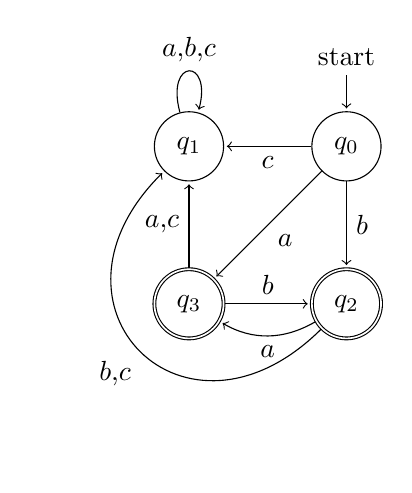
\begin{tikzpicture}[node distance=2cm,shorten >=1pt,auto]
\node[state,initial,initial where=above]   (q_0)                {$q_0$};
\node[state]           (q_1) [left of=q_0]  {$q_1$};
\node[state,accepting] (q_2) [below of=q_0] {$q_2$};
\node[state,accepting] (q_3) [left of=q_2]  {$q_3$};
\path[->]	(q_0) 	edge 			node {$b$} 		(q_2)
			edge 			node {$c$} 		(q_1)
			edge 			node {$a$} 		(q_3)
		(q_1)	edge [loop above]	node {$a$,$b$,$c$}	()
		(q_2)	edge [bend left]	node {$a$}		(q_3)
			edge [bend left=90,looseness=2.2]	node {$b$,$c$}		(q_1)
		(q_3)	edge			node {$a$,$c$}		(q_1)
			edge			node {$b$}		(q_2);
\end{tikzpicture}
\end{center}
\end{enumerate}
\end{frame}
\begin{frame}
	\begin{enumerate}
	\setcounter{enumi}{2}
	\item Aufgabe: Konstruiere einen DEA der alle durch 5 teilbaren Zahlen akzeptiert. Als Eingabe erhält der Automat dabei die Zahl in ihrer binären Darstellung. Also ist $\Sigma = \{0, 1\}$. Z.B. soll Automat $10_{10} = 1010_{2}$ akzeptieren, aber $7_{10} = 111_{2}$ ablehnen.
	\pause \\[10pt]
	Tip: Restklassen als Zustände modellieren
	\end{enumerate}
\end{frame}
\begin{frame}
	\frametitle{DEA: Lösung}
	\begin{enumerate}
	\setcounter{enumi}{2}
	\item Idee
		\begin{itemize}
		\item $Q = (q_0, q_1, q_2, q_3, q_4)$\\
		\item $\Sigma = \{0,1\}$
		\item $\delta(q_n, c) \rightarrow q_{n \cdot 2 + c\mbox{ mod }5}$ mit $c\in\Sigma$\\
		\item $S = q_0$\\
		\item $F = \{q_0\}$
		\end{itemize}
	\end{enumerate}
\end{frame}
\subsection{Nichtdeterministische endliche Automaten}
\begin{frame}
\frametitle{Nichtdeterministische Endliche Automaten}
        Ein nichtdeterministischer endlicher Automat $M$ ist ein 5-Tupel
        \[
        M= (Q,\Sigma,\delta,S,F).
        \]
        \begin{itemize}
        \item $Q$:  endliche Zustandsmenge
        \item $\Sigma$:    endliches Alphabet
        \item \textcolor{red}{$\delta$:   Zustandsübergangsfunktion $Q\times (\Sigma \cup \varepsilon) \rightarrow 2^Q$}
        \item $S$:   Startzustand $\in Q$
        \item $F$:   Endzustandsmenge $\subseteq Q$
        \end{itemize}
	Damit der NEA ein Wort akzeptiert, muss es \emph{einen} akzeptierenden Weg geben.
\end{frame}
\begin{frame}
	\frametitle{NEA: Beispiel}
	\begin{figure}
	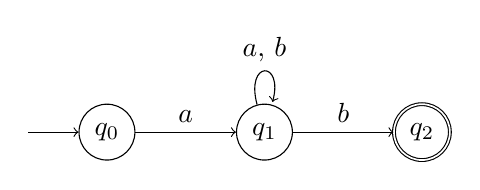
\begin{tikzpicture}
	\node[draw,circle] (q_0) at (0,0) {$q_0$};
	\node[draw,circle] (q_1) at (2,0) {$q_1$};
	\node[draw,circle,double] (q_2) at (4,0) {$q_2$};
	\draw[->] (-1,0) -- (q_0);
	\draw[->] (q_0) -- (q_1) node[midway,anchor=south] {$a$};
	\draw[->] (q_1) -- (q_2) node[midway,anchor=south] {$b$};
	\draw (q_1) edge [loop above] node {$a$, $b$} (q_1);
	\end{tikzpicture}
	\end{figure}
	Bei Eingabe von $b$ im Zustand $q_1$ gibt es mehrere Möglichkeiten.
\end{frame}
\begin{frame}
	\frametitle{NEA: Aufgabe}
 Welche Sprache akzeptiert der nichtdeterministische endliche Automat
 zu dem folgenden Zustandsgraphen?
\begin{center}
\vspace{-0.7cm}
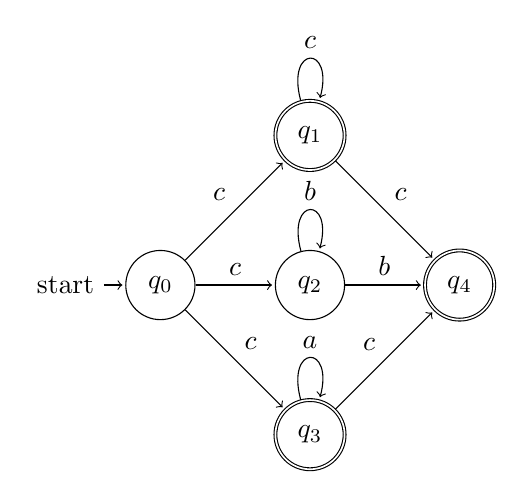
\begin{tikzpicture}[scale=0.6,node distance=1.9cm,shorten >=1pt,auto]
\node[state,initial]   (q_0)                {$q_0$};
\node[state]           (q_2) [right of=q_0]  {$q_2$};
\node[state,accepting] (q_1) [above of=q_2] {$q_1$};
\node[state,accepting] (q_3) [below of=q_2]  {$q_3$};
\node[state,accepting] (q_4) [right of=q_2]  {$q_4$};
\path[->]	(q_0) 	edge 			node {$c$} 		(q_1)
			edge 			node {$c$} 		(q_2)
			edge 			node {$c$} 		(q_3)
		(q_1)	edge [loop above]	node {$c$}		()
			edge 			node {$c$}		(q_4)
		(q_2)	edge [loop above]	node {$b$}		()
			edge 			node {$b$}		(q_4)
		(q_3)	edge [loop above]	node {$a$}		()
			edge			node {$c$}		(q_4);
\end{tikzpicture}
\end{center}
\end{frame}

\subsubsection{Potenzmengenkonstruktion}
\frame{
\frametitle{Potenzmengenkonstruktion}
Jeder nichtdeterministische endliche Automat hat einen äquivalenten deterministischen endlichen Automat.
 \begin{figure}[H]
 \begin{center}
 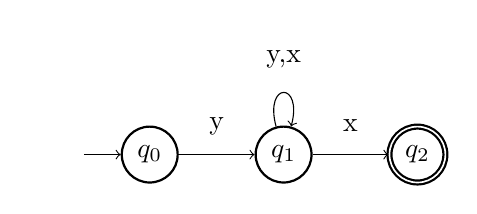
\begin{tikzpicture}[node distance=1.7cm]
 \tikzstyle{every node}=[circle, thick, minimum size = 7mm]
 \tikzstyle{normal}=[draw]
 \node[normal] 	(q0)		{$q_0$};
 \node[normal] 	(q1)	[right of=q0] {$q_1$};
 \node[normal,double]		(q2)	[right of=q1]{$q_2$};
 \node 		(s) 	[left of =q0, xshift=0.5cm]	{};
 
 \draw[->](s) to (q0);
 \draw[->](q0) to node[above]{y} (q1);
 \draw[->, loop above](q1) to node[above]{y,x} (q1);
 \draw[->](q1) to node[above]{x} (q2);x
 \end{tikzpicture}
 \end{center}
 \end{figure}
In eine Tabelle werden die Automatenzustände und ihre Folgezustände bei jeweiliger Eingabe eingetragen. \\
\begin{center}
\vspace{-6pt}
\begin{tabular}{l|l|l}
    & y & x \\
\hline
 $\{q_0\}$ 	&	 $\{q_1\}$	&	$\emptyset$ \\
 $\{q_1\}$	&	$\{q_1\}$	&	$\textcolor{red}{\{q_1, q2 \}}$\\
\end{tabular}
\end{center}
}
\frame{
\frametitle{Potenzmengenkonstruktion}
Ein \textcolor{red}{neuer Zustand} entsteht, wenn man von einem alten Zustand durch eine Eingabe in mehrere Zustände kommt.
\vspace{-0.3cm}
\begin{center}
\begin{tabular}{l|l|l}
    & y & x \\
\hline
 $\{q_0\}$ 	&	 $\{q_1\}$	&	$\emptyset$ \\
 $\{q_1\}$	&	$\{q_1\}$	&	$\textcolor{red}{\{q_1, q_2\}}$\\ \
 $\textcolor{red}{\{q_1, q_2\}}$ & 	$\{q_1\}$	&	$\{q_1, q_2\}$\\
 $\emptyset$	&	$\emptyset$		& 	$\emptyset$
\end{tabular}
\end{center}
\vspace{-1cm}
\begin{figure}[H]
\begin{center}
 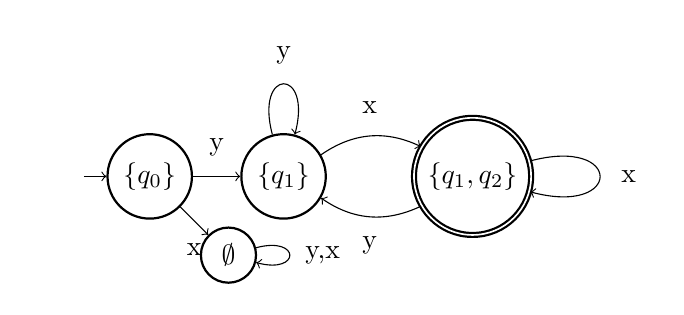
\begin{tikzpicture}[node distance=1.7cm]
 \tikzstyle{every node}=[circle, thick, minimum size = 7mm]
 \tikzstyle{normal}=[draw]
 \node[normal] 	(q0)		{\{$q_0$\}};
 \node[normal] 	(q1)	[right of=q0] {\{$q_1$\}};
 \node[normal,double,node distance=2.4cm]		(q2)	[right of=q1]{\{$q_1, q_2$\}};
 \node[normal]	(f) at (1,-1)	{$\emptyset$};
 \node 		(s) 	[left of =q0, xshift=0.5cm]	{};
  \draw[->](q0) to node[above]{y}(q1);
  \draw[->](s) to (q0);
  \draw[->](q0) to node[below]{x}(f);
  \draw[->,loop above](q1) to node[above]{y}(q1);
  \draw[->,bend left](q1) to node[above]{x}(q2);
  \draw[->, bend left](q2) to node[below]{y}(q1);
  \draw[->, loop right](q2) to node[right]{x}(q2);
  \draw[->, loop right](f) to node[right]{y,x}(f);
\end{tikzpicture}
\end{center}
\end{figure}

}
\frame{
\frametitle{Potenzmengenkonstruktion}
Die Einträge der ersten Spalte sind die neuen Zustände. Alle Mengen die einen Endzustand enthalten, sind wiederum im neuen Automaten Endzustände
\begin{figure}[H]
\begin{center}
 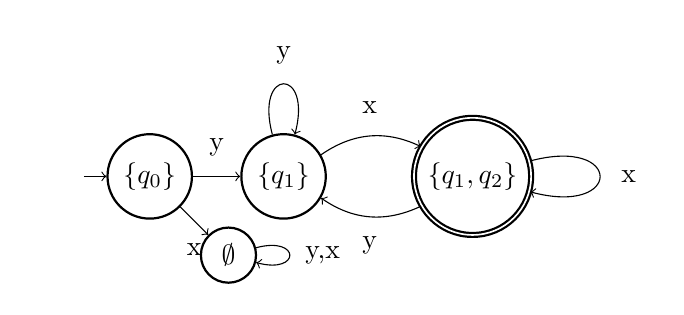
\begin{tikzpicture}[node distance=1.7cm]
 \tikzstyle{every node}=[circle, thick, minimum size = 7mm]
 \tikzstyle{normal}=[draw]
 \node[normal] 	(q0)		{\{$q_0$\}};
 \node[normal] 	(q1)	[right of=q0] {\{$q_1$\}};
 \node[normal,double,node distance=2.4cm]		(q2)	[right of=q1]{\{$q_1, q_2$\}};
 \node[normal]	(f) at (1,-1)	{$\emptyset$};
 \node 		(s) 	[left of =q0, xshift=0.5cm]	{};
  \draw[->](q0) to node[above]{y}(q1);
  \draw[->](s) to (q0);
  \draw[->](q0) to node[below]{x}(f);
  \draw[->,loop above](q1) to node[above]{y}(q1);
  \draw[->,bend left](q1) to node[above]{x}(q2);
  \draw[->, bend left](q2) to node[below]{y}(q1);
  \draw[->, loop right](q2) to node[right]{x}(q2);
  \draw[->, loop right](f) to node[right]{y,x}(f);
\end{tikzpicture}
\end{center}
\end{figure}

}
\subsection{Konstruktion eines DEA aus einem NEA}
\begin{frame}
  \frametitle{NEA2DEA: Aufgaben}
  Über dem Alphabet $\Sigma = \{a,b\}$ sei der reguläre
  Ausdruck
  $r := {(a \cup (ab (b)^* ba))^*}$
  gegeben.
  \begin{enumerate}
    \setlength{\itemsep}{0ex}
  \item Geben Sie einen NEA an, der $L(r)$ erkennt. Begründen Sie
    kurz die Korrektheit Ihres Automaten, ein formaler
    Korrektheitsbeweis ist jedoch nicht erforderlich.\\
    (Hinweis: Es gibt einen NEA mit 3 Zuständen.)
  \item Konstruieren Sie zu dem von Ihnen angegebenen NEA einen
    äquivalenten DEA mittels Potenzmengenkonstruktion.
  \end{enumerate}
\end{frame}


\begin{frame}
	\frametitle{Eliminierung von $\varepsilon$-Übergängen}
	\begin{block}{Satz 2.13 (Skript)}
	\begin{itemize}
	 \item Zu jedem nichtdeterministischen endlichen Automaten mit \(\varepsilon\)-Übergängen gibt es einen äquivalenten nichtdeterministischen
	 endlichen Automaten ohne \(\varepsilon\)-Übergänge, der nicht mehr Zustände hat.
	 \item äquivalent = akzeptiert die selbe Sprache.
	\end{itemize}
	\end{block}
	\begin{block}{Erinnerung}
		Der \(\varepsilon\)-Abschluss $E(q)$ eines Zustandes $q$ ist definiert als die Menge aller Zustände, die von $q$ aus durch lediglich \(\varepsilon\)-Übergänge erreichbar sind. ($q$ selbst zählt auch dazu)
	\end{block}
\end{frame}
\begin{frame}
\frametitle{Eliminierung von $\varepsilon$-Übergängen}
	\begin{block}{Konstruktion}
	Zu einem NEA \(A := (Q, \Sigma, \delta, s, F)\) mit \(\varepsilon\)-Übergängen konstruieren wir einen 
	  äquivalenten NEA \(\tilde{A} := (\tilde{Q}, \Sigma, \tilde{\delta}, \tilde{s}, \tilde{F})\) mit
	 \begin{itemize}
	 \item \(\tilde{Q} := Q\)
	 \item \(\tilde{s} := s\)
	 \item \(\tilde{F} := \{q|E(q)\cap F \neq \emptyset\}\)
	 \item \[\tilde{\delta}(q,a) := 
	 \begin{cases}
	  \{q\}			& \text{falls $a = \varepsilon$} \\
	 \delta(E(q),a)	& \text{sonst}
	 \end{cases}\]
	 \end{itemize}
	\end{block}
	\begin{block}{Eigenschaften von \(\tilde{A}\)}
	 \(L(\tilde{A}) = L(A)\), und \(|\tilde{Q}| = |Q|\).
	\end{block}

\end{frame}
\begin{frame}
	\frametitle{NEA2DEA: Aufgaben}
Gegeben sei der NEA ${\cal A}=(\{s,q,f\},\{a,b,c\},\delta,s,\{f\})$, wobei
die Übergangsfunktion $\delta$ gegeben ist durch:
\begin{center}
$\begin{array}{r|cccc}
&\varepsilon & a & b & c\\\hline
s & \{q,f\} & \emptyset & \{q\} &\{f\}\\
q &  \emptyset & \{s\} & \{f\} & \{s,q\}\\
f & \emptyset & \emptyset &  \emptyset &  \emptyset\\
\end{array}$
\end{center}
\begin{enumerate}
\item Geben Sie zu dem Automaten ${\cal A}$ den Übergangsgraphen an und eliminieren
Sie die $\varepsilon$-Übergänge.
\item Ermitteln Sie mittels Potenzmengenkonstruktion den zu ${\cal A}$ äquivalenten
DEA. Geben Sie hierbei die Übergangsfunktion tabellarisch an.
\end{enumerate}
\end{frame}
\begin{frame}	
\frametitle{Aufgaben zu \(\varepsilon\)-Übergängen}
Sei $A=(Q,\Sigma, \delta, s, \{q_f\})$ ein NEA, derart dass es keine zu $s$ hinführenden und keine von $q_f$ ausgehenden Übergänge gibt. Beschreiben Sie für jede der folgenden Modifikationen von A die akzeptierte Sprache als Modifikation von $L=L(A)$:
\begin{enumerate}
\item Der Automat, der aus A konstruiert wird, indem $\varepsilon$-Übergänge von $s$ zu jedem Zustand hinzugefügt werden, der von $s$ aus auf einem Pfad erreichbar ist, dessen Beschriftungen sowohl Symbole aus $\Sigma$ als auch $\varepsilon$ enthalten können.
\item Der Automat, der aus A konstruiert wird, indem von jedem Zustand $\varepsilon$-Übergänge nach $q_f$ hinzugefügt werden, von dem aus $q_f$ auf irgendeinem Pfad erreichbar ist.
\item Der Automat, der aus A konstruiert wird, indem die unter (1) und (2) geforderten Modifikationen ausgeführt werden.
\end{enumerate}

\end{frame}

\subsection{Konstruktion eines regulären Ausdrucks}
\begin{frame}
\frametitle{Konstruktion eines RA aus einem DEA}
Wir wissen, jeder DEA hat einen Regulären Ausdruck, der genau die Sprache beschreibt, die der Automat akzeptiert, wie konstruiert man nun diesen RA aus dem DEA?\\[0.6cm]
\textbf{Idee:} Betrachte die Sprachen $L_{q_r,i,q_t}$, definiert als \( w \in \Sigma^*\) mit $w$ überführt $q_r$ in $q_t$ unter Benutzung der Zwischenzustände $\{q_1,\ldots,q_i\}$
\begin{itemize}
\item Es ist $L = \cup_{f\in F} L_{s,n,f}$
\item Es ist weiterhin $L_{q_r,i+1,q_t} = L_{q_r,i,q_t} \cup (L_{q_r,i,q_{i+1}}(L_{q_{i+1},i,q_{i+1}})^*L_{q_{i+1},i,q_t})$
\item Letztlich ist: $L_{q_r, 0, q_t}$ immer regulär, das sind die Zeichen mit denen man ohne weitere Zustände zu verwenden von $q_r$ nach $q_t$ kommt (sowie $\varepsilon$ falls $r = t$).
\item Unter Benutzung dieser Punkte, kann man nun einen Regulären Ausdruck zu einem DEA Konstruieren.
\end{itemize}
\end{frame}
\begin{frame}
\frametitle{Beispiele zum Verständnis}
\vspace{-1cm}
\begin{figure}[H]
\begin{center}
\begin{tikzpicture}[scale=0.6,node distance=1.9cm,shorten >=1pt,auto]
\node[state,initial]   (q_1)                {$q_1$};
\node[state,accepting] (q_2) [right of=q_0] {$q_2$};
\path[->]	(q_1) 	edge 			node {$0$} 		(q_2)
			edge [loop above]	node {$1$}		()
		(q_2)	edge [loop above]	node {$0$,$1$}		();
\end{tikzpicture}
\end{center}
\end{figure}
Was sind hier jeweils:
\begin{itemize}
\item $L_{q_1,0,q_1}$\pause $ = (1\cup\varepsilon)$
\item $L_{q_1,0,q_2}$\pause $ = (0)$
\item $L_{q_1,1,q_1}$\pause $ = (1^*)$
\item $L_{q_2,1,q_2}$\pause $ = (0\cup1\cup\varepsilon)$
\item $L_{q_2,2,q_2}$\pause $ = (0\cup1)^*$
\item $L_{q_1,2,q_2}$\pause $ = 1^*0(0\cup1)^*$
\end{itemize}
\end{frame}

\begin{frame}
\frametitle{Ausführliche Konstruktion}
\vspace{-1cm}
\begin{figure}[H]
\begin{center}
\begin{tikzpicture}[scale=0.6,node distance=1.9cm,shorten >=1pt,auto]
\node[state,initial]   (q_1)                {$q_1$};
\node[state,accepting] (q_2) [right of=q_0] {$q_2$};
\path[->]	(q_1) 	edge 			node {$0$} 		(q_2)
			edge [loop above]	node {$1$}		()
		(q_2)	edge [loop above]	node {$0$,$1$}		();
\end{tikzpicture}
\end{center}
\end{figure}
\begin{enumerate}
\item $L_{q_1,2,q_2} = L_{q_1,1,q_2}\cup(L_{q_1,1,q_2}(L_{q_2,1,q_2})^*L_{q_2,1,q_2})$
\item $L_{q_1,1,q_2} = L_{q_1,0,q_2}\cup(L_{q_1,0,q_1}(L_{q_1,0,q_1})^*L_{q_1,0,q_2}) = 0\cup((1\cup\varepsilon)(1\cup\varepsilon)^*0)$
\item $L_{q_2,1,q_2} = L_{q_2,0,q_2}\cup(L_{q_2,0,q_1}(L_{q_1,0,q_1})^*L_{q_1,0,q_2})$ $ = (0\cup1\cup\varepsilon)$
\item Also: $L_{q_1,2,q_2} = 0\cup(1\cup\varepsilon)(1\cup\varepsilon)^*0\cup((0\cup((1\cup\varepsilon)(1\cup\varepsilon)^*0))(0\cup1\cup\varepsilon)^*(0\cup1\cup\varepsilon))$
\item Vereinfacht: $1^*0(0\cup1)^*$
\end{enumerate}
\end{frame}

\begin{frame}
\frametitle{Aufgabe}
Bestimmen Sie  mit dem im Beweis von Satz 2.14 verwendeten Verfahren die 
reguläre Sprache, die folgender deterministische endliche Automat erkennt:
\begin{figure}[H]
\begin{center}
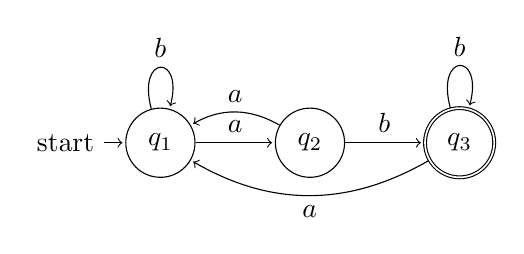
\begin{tikzpicture}[scale=0.6,node distance=1.9cm,shorten >=1pt,auto]
\node[state,initial]   (q_1)                {$q_1$};
\node[state] (q_2) [right of=q_1] {$q_2$};
\node[state,accepting] (q_3) [right of=q_2] {$q_3$};

\path[->]	(q_1) 	edge 			node {$a$} 		(q_2)
			edge [loop above]	node {$b$}		()
		(q_2)	edge [bend right]	node [above] {$a$}		(q_1)
			edge 			node {$b$}		(q_3)
		(q_3)	edge [loop above]	node {$b$}		()
			edge [bend left]	node {$a$}		(q_1);
\end{tikzpicture}
\end{center}
\end{figure}
\end{frame}

%Pumpin' Lemma
\begin{frame}
\frametitle{Pumping Lemma}
\begin{exampleblock}{Pumping Lemma}
Sei $L$ eine reguläre Sprache, dann existiert eine Zahl $n \in \mathbb{N}$, so dass für jedes wort $w \in L$ mit $\left|w \right| > n$ eine Darstellung $$w = uvx$$ existiert, so dass folgende Eigenschaften erfüllt sind:

\begin{enumerate}
\item $v \neq \varepsilon$ 
\item $\left|uv\right| \leq n$ 
\end{enumerate}
So folgt: Für alle $i \in \mathbb{N}_0$ gilt: $uv^ix \in L$
\end{exampleblock}
\end{frame}
\begin{frame}
\frametitle{Pumping Lemma: Übersicht}
\begin{itemize}
\item Für jede Reguläre Sprache gilt das Pumping-Lemma, nicht jede Sprache für die das Pumping-Lemma gilt ist regulär!
\item In der Übung wird üblicherweise die Kontraposition des Pumping-Lemmas verwendet. Man zeigt für eine Sprache, dass das Pumping-Lemma \emph{nicht} erfüllt ist, und daraus folgt, dass diese Sprache \emph{nicht} regulär sein kann.
\begin{itemize}
\item Konkret: Finden wir für \emph{jedes} $n$ \emph{ein} $w$ mit $\left|w\right| > n$, so dass für \emph{jede} Darstellung $w = uvx$ mit $v \neq \varepsilon$ sowie $\left|uv\right| \leq n$, ein $i \in \mathbb{N}_0$ mit $uv^ix \notin L$, dann ist $L$ nicht regulär.
\item \textbf{Wichtig:} Alle Quantoren werden umgekehrt.
\end{itemize}
\end{itemize}
\end{frame}

\begin{frame}
\frametitle{Beispiel}
Sei $\Sigma = \{a, b\}$ und $L = \{a^nb^n\,|\,n\geq0\}$. (Also $L = \{\varepsilon,ab, aabb, aaabbb, \ldots\}$)
\begin{enumerate}
\item Für ein $n$ wähle das Wort $w = a^nb^n$.
\item Es ist also $\left|w\right| > n$.
\item Nun ist aber für \emph{jede} Darstellung $w = uvx$ mit $\left|uv\right| \leq n$ und $v \neq \varepsilon$ $v = a^m$ mit $m \geq 0$. Demnach ist $uv^0x = a^lb^n \neq L$, da $l < n$.
\item Daher kann $L$ nicht regulär sein.
\end{enumerate}

\end{frame}

\begin{frame}
\frametitle{Pumping Lemma: Aufgaben}
Welche der folgenden Sprachen sind regulär? Begründen Sie Ihre Antwort.

\begin{enumerate}
\item $L=\{a^kc^lb^k \mid k, l \geq 0 \}$
\item Die Menge aller Wörter über $\{0, 1\}$, sodass auf jede Null eine Eins folgt
\item Die Menge der Wörter über $\{0, 1\}$, die die Form $w\bar{w}$ haben, wobei $\bar{w}$ aus $w$ gebildet
wird, indem alle Nullen durch Einsen und alle Einsen durch Nullen ersetzt werden; so ist etwa 
$\overline{011}=100$ und $011100$ ein Beispiel für ein Wort dieser Sprache
\end{enumerate}

\end{frame}

\subsection{Minimierung und Äquivalenzklassenautomat}
%Der Automat hier ist vom vorherigen Beispiel kopiert, aber er sollte den Zweck erfüllen.
\begin{frame}
 \frametitle{Minimierung von DEAs}
 \begin{block}{Beispielautomat \(A = (Q, \Sigma, \delta, s, F)\)}
 \begin{figure}[H]
\begin{center}
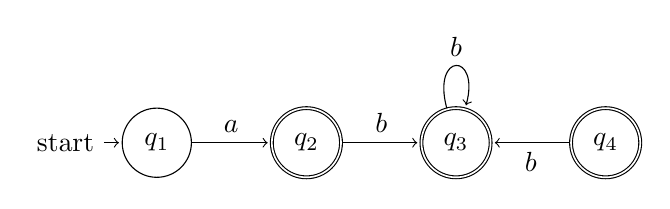
\begin{tikzpicture}[scale=0.5,node distance=1.9cm,shorten >=1pt,auto]
\node[state,initial]   (q_1)                {$q_1$};
\node[state,accepting] (q_2) [right of=q_1] {$q_2$};
\node[state,accepting] (q_3) [right of=q_2] {$q_3$};
\node[state,accepting] (q_4) [right of=q_3] {$q_4$};

\path[->]	(q_1) 	edge 			node {$a$} 		(q_2)
		(q_2)	edge 			node {$b$}		(q_3)
		(q_3)	edge [loop above]	node {$b$}		()
		(q_4)	edge			node {$b$}		(q_3);
\end{tikzpicture}
\end{center}
\end{figure}
\end{block}
Kann $A$ auf einen Automaten $A' = (Q', \Sigma, \delta', s', F')$ mit $L(A) = L(A')$ und $|Q'| \le |Q|$ überführt werden?
\end{frame}
\begin{frame}
\frametitle{Minimierung von DEAs}
$q_4$ ist nicht vom Startzustand aus erreichbar
\begin{block}{Entferne \(q_4\)}
 \begin{figure}[h]
\begin{center}
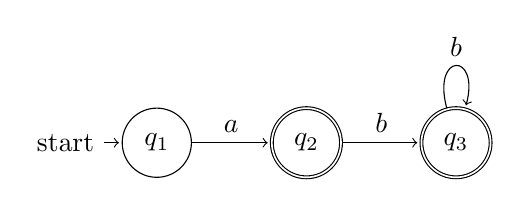
\begin{tikzpicture}[scale=0.5,node distance=1.9cm,shorten >=1pt,auto]
\node[state,initial]   (q_1)                {$q_1$};
\node[state,accepting] (q_2) [right of=q_1] {$q_2$};
\node[state,accepting] (q_3) [right of=q_2] {$q_3$};

\path[->]	(q_1) 	edge 			node {$a$} 		(q_2)
		(q_2)	edge 			node {$b$}		(q_3)
		(q_3)	edge [loop above]	node {$b$}		();
\end{tikzpicture}
\end{center}
\end{figure}
\end{block}
\pause
Schon minimal?
\end{frame}
\begin{frame}
Nein!
\begin{block}{Automat \(A'' = (Q'', \Sigma, \delta'', s, F'')\)}
 \begin{figure}[H]
\begin{center}
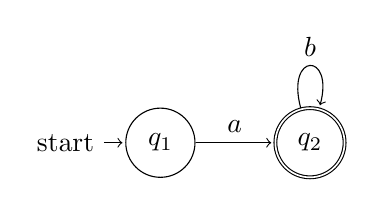
\begin{tikzpicture}[scale=0.6,node distance=1.9cm,shorten >=1pt,auto]
\node[state,initial]   (q_1)                {$q_1$};
\node[state,accepting] (q_2) [right of=q_1] {$q_2$};

\path[->]	(q_1) 	edge 			node {$a$} 		(q_2)
		(q_2)	edge [loop above]	node {$b$}		();
\end{tikzpicture}
\end{center}
\end{figure}
\end{block}
\begin{block}{}
 Akzeptierte Sprache: \(L(A) = L(A') = L(A'') = L(ab^*) \)
\end{block}
\end{frame}
\begin{frame}
 \frametitle{Methodischer Ansatz}
 \begin{block}{Definition}
  Zustände eines (deterministischen) endlichen Automaten, die vom Anfangszustand aus nicht erreichbar sind, heißen überflüssig.
 \end{block}
\begin{block}{Vorgehen}
 \begin{enumerate}
  \item Tiefensuche durchführen um nicht erreichbare Zustände zu finden.
  \item Diese entfernen.
  \item Aus den restlichen Zuständen den Äquivalenzklassenautomaten bilden.
 \end{enumerate}
\end{block}
\end{frame}
\begin{frame}
 \frametitle{Äquivalenz}
 \vspace{-1cm}
 \begin{block}{Aus der Vorlesung}
  \begin{itemize}
   \item Zwei Zustände haben dasselbe Akzeptanzverhalten, wenn es für das Erreichen eines Endzustandes durch Abarbeiten eines Wortes $w$
   unerheblich ist, aus welchem der beiden Zustände wir starten.
  \end{itemize}
 \end{block}
 \begin{block}{Definition (Äquivalenz):}
  Zwei Zustände $p$ und $q$ eines deterministischen endlichen Automaten heißen \emph{äquivalent} ($p \equiv $q),
  wenn für alle Wörter $w\in\Sigma^*$ gilt:
  \[
   \delta(p, w)\in F \leftrightarrow \delta(q, w)\in F
  \]
  Offensichtlich ist $\equiv$ eine Äquivalenzrelation. Mit $[p]$ bezeichnen wir die Äquivalenzklasse der zu $p$ äquivalenten Zustände.
 \end{block}
\end{frame}
\begin{frame}
 \frametitle{Beispiel}
 \begin{block}{Zurück zu $Q'$}
 \begin{figure}[h]
\begin{center}
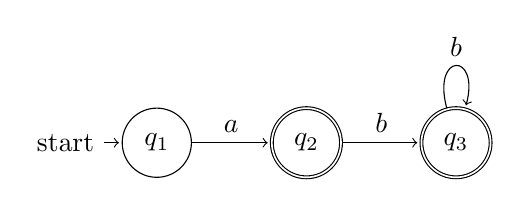
\begin{tikzpicture}[scale=0.5,node distance=1.9cm,shorten >=1pt,auto]
\node[state,initial]   (q_1)                {$q_1$};
\node[state,accepting] (q_2) [right of=q_1] {$q_2$};
\node[state,accepting] (q_3) [right of=q_2] {$q_3$};

\path[->]	(q_1) 	edge 			node {$a$} 		(q_2)
		(q_2)	edge 			node {$b$}		(q_3)
		(q_3)	edge [loop above]	node {$b$}		();
\end{tikzpicture}
\end{center}
\end{figure}
Hier sind $q_2$ und $q_3$ äquivalent. Warum?
\end{block}
\end{frame}
\begin{frame}
 \frametitle{Äquivalenzklassenautomat}
 \begin{block}{Definition aus der Vorlesung (Äquivalenzklassenautomat)}
  Zu einem DEA \(A = (Q, \Sigma, \delta, s, F)\) definieren wir den Äquivalenzklassenautomaten 
  \(A^\equiv = (Q^\equiv, \Sigma^\equiv, \delta^\equiv, s^\equiv, F^\equiv)\) durch:
  \begin{itemize}
   \item $Q^\equiv := \{[q]|q\in Q\}$
   \item $\Sigma^\equiv := \Sigma$
   \item $\delta\equiv([q], a) := [\delta(q, a)]$
   \item $s\equiv := [s]$
   \item $F\equiv:= \{[f]|f\in F\}$
  \end{itemize}
 \end{block}
\end{frame}
\begin{frame}
 \frametitle{Konstruktion der Äquivalenzklassen}
 \begin{block}{}
  \begin{enumerate}
   \item Fasse alle Zustände $q_i \in Q$ in eine Klasse zusammen.
   \item $\varepsilon$ trennt Zustände aus $F$ von denen aus $Q \backslash F$
   \item Für Zustandspaare $p, q$ in einer Klasse und
   Worte $w\in \Sigma^*$ mit wachsender Länge: 
    \begin{enumerate}
    \item falls $[\delta(p, w)] != [\delta(q, w)]$ trenne die Zustände $q$ und $p$. (w ist Zeuge)
    \item breche ab falls sich für eine Wortlänge keine weiteren Zeugen finden.
    \end{enumerate}
  \end{enumerate}
 \end{block}
\end{frame}
\begin{frame}
 \frametitle{Beispiel $Q'$}
 \vspace{-1cm}
 \begin{figure}[h]
\begin{center}
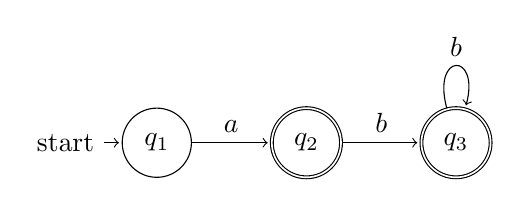
\begin{tikzpicture}[scale=0.5,node distance=1.9cm,shorten >=1pt,auto]
\node[state,initial]   (q_1)                {$q_1$};
\node[state,accepting] (q_2) [right of=q_1] {$q_2$};
\node[state,accepting] (q_3) [right of=q_2] {$q_3$};

\path[->]	(q_1) 	edge 			node {$a$} 		(q_2)
		(q_2)	edge 			node {$b$}		(q_3)
		(q_3)	edge [loop above]	node {$b$}		();
\end{tikzpicture}
\end{center}
\end{figure}
 \begin{block}{Anfangs}
  $\{q_1, q_2, q_3\}$
 \end{block}
 \pause
 \begin{block}{Zeugen der Länge 0: $\varepsilon$}
  $\{q_1\} \{q_2, q_3\}$
 \end{block}
  \pause
  \begin{block}{Zeugen der Länge 1: a, b}
   $a$ oder $b$ trennen keine Zustände mehr voneinander $\rightarrow$ Abbruch.
  \end{block}
\end{frame}

\frame{
  \frametitle{Automaten-Minimierung: Beispiel, Methode 1}
%   \begin{center}
%   (Benötigt wird ein vollständiger DEA.)
%   \end{center}
  \begin{figure}[H]
  \begin{center}
  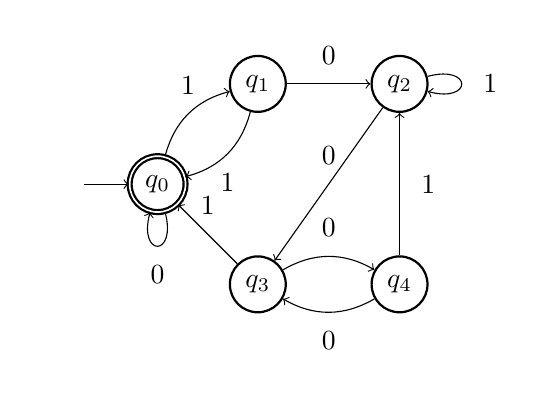
\begin{tikzpicture}[node distance=1.8cm]
  \tikzstyle{every node}=[circle,thick,minimum size=7mm]
  \tikzstyle{normal}=[draw]


  \node[normal,double]  (q0)                      {$q_0$};
  \node[normal]         (q1)  [above right of=q0] {$q_1$};
  \node[normal]         (q2)  [right of=q1]       {$q_2$};
  \node[normal]         (q3)  [below right of=q0] {$q_3$};
  \node[normal]         (q4)  [right of=q3]       {$q_4$};
  
  \node (start) [left of=q0,xshift=0.5cm] {};
  
  \draw[->] (start) to (q0);

  \draw[->,bend left] (q0)  to node[above] {1} (q1);
  \draw[->,loop below] (q0)  to node [below] {0} (q0);

  \draw[->,bend left] (q1)  to node[below] {1} (q0);
  \draw[->] (q1)  to node[above] {0} (q2);

  \draw[->] (q2) to node[above] {0} (q3);
  \draw[->,loop right] (q2) to node[right] {1} (q2);

  \draw[->] (q3)  to node[above] {1} (q0);
  \draw[->,bend left] (q3)  to node[above] {0} (q4);
  
  \draw[->,bend left] (q4)  to node[below] {0} (q3);
  \draw[->] (q4)  to node[right] {1} (q2);

  \end{tikzpicture}
  \end{center}
  \end{figure}
}

\frame{
  \frametitle{Minimierung, Ausführlicheres Beispiel/Aufgabe}
  \begin{figure}[H]
  \begin{center}
  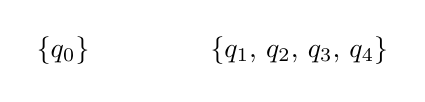
\begin{tikzpicture}

  \node (a0) {$\{q_0\}$};
  \node[right of=a0,xshift=2cm] (b0) {\{$q_1$, $q_2$, $q_3$, $q_4$\}};

  \end{tikzpicture}
  \end{center}
  \end{figure}
}

\frame{
  \frametitle{Minimierung, Ausführlicheres Beispiel}
  \begin{figure}[H]
  \begin{center}
  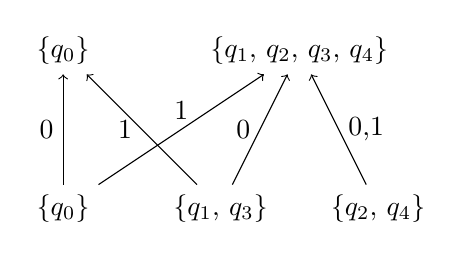
\begin{tikzpicture}

  \node (a0) {$\{q_0\}$};
  \node[right of=a0,xshift=2cm] (b0) {\{$q_1$, $q_2$, $q_3$, $q_4$\}};

  \node[below of=a0,yshift=-1cm] (a1) {$\{q_0\}$};
  \node[right of=a1,xshift=1cm] (b1) {\{$q_1$, $q_3$\}};
  \node[right of=b1,xshift=1cm] (c1) {\{$q_2$, $q_4$\}};

  \draw[->] (a1) to node[left] {0} (a0);
  \draw[->] (a1) to node[above] {1} (b0);
  \draw[->] (b1) to node[left] {1} (a0);
  \draw[->] (b1) to node[left] {0} (b0);
  \draw[->] (c1) to node[right] {0,1} (b0);

  \end{tikzpicture}
  \end{center}
  \end{figure}
}
\frame{
  \frametitle{Minimierung, Ausführlicheres Beispiel}
  \begin{figure}[H]
  \begin{center}
  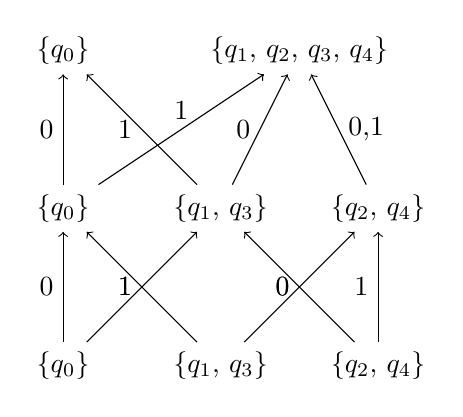
\begin{tikzpicture}

  \node (a0) {$\{q_0\}$};
  \node[right of=a0,xshift=2cm] (b0) {\{$q_1$, $q_2$, $q_3$, $q_4$\}};

  \node[below of=a0,yshift=-1cm] (a1) {$\{q_0\}$};
  \node[right of=a1,xshift=1cm] (b1) {\{$q_1$, $q_3$\}};
  \node[right of=b1,xshift=1cm] (c1) {\{$q_2$, $q_4$\}};

  \node[below of=a1,yshift=-1cm] (a2) {$\{q_0\}$};
  \node[right of=a2,xshift=1cm] (b2) {\{$q_1$, $q_3$\}};
  \node[right of=b2,xshift=1cm] (c2) {\{$q_2$, $q_4$\}};

  \draw[->] (a1) to node[left] {0} (a0);
  \draw[->] (a1) to node[above] {1} (b0);
  \draw[->] (b1) to node[left] {1} (a0);
  \draw[->] (b1) to node[left] {0} (b0);
  \draw[->] (c1) to node[right] {0,1} (b0);

  \draw[->] (a2) to node[left] {0} (a1);
  \draw[->] (a2) to node[left] {1} (b1);
  \draw[->] (b2) to node[left] {0} (c1);
  \draw[->] (b2) to node[left] {1} (a1);
  \draw[->] (c2) to node[left] {0} (b1);
  \draw[->] (c2) to node[left] {1} (c1);

  \end{tikzpicture}
  \end{center}
  \end{figure}
}


\subsection{Nerode-Relation}
\begin{frame}
 \frametitle{Nerode-Relation}
 \begin{block}{Definition 2.25}
 Für eine Sprache \(L \subseteq \Sigma^*\) ist die \emph{Nerode-Relation} \(R_L\) definiert durch:
  
  für \(x, y \in \Sigma^*\) ist $x$ $R_L$ $y$ genau dann wenn \((xz \in L \leftrightarrow yz \in L)\) für alle $z \in \Sigma^*$ gilt.
 \end{block}
  \begin{block}{Erinnerung}
   Die minimale Anzahl an Zuständen eines endlichen Automaten einer Sprache $L \subseteq \Sigma^*$ entspricht dem Index der Nerode-Relation.
  \end{block}
\end{frame}
\begin{frame}
\frametitle{Aufgabe zur Nerode-Relation}
Bestimmen Sie die Äquivalenzklassen der Nerode-Relation zur Sprache $L=\{a^ib^jc^k \mid i,j,k \in \mathbb{N}_{>0} \}$ über dem Alphabet $\Sigma=\{a,b,c\}$.
\end{frame}
\begin{frame}
 Sei $\Sigma = \{a,b,c\}.$ Geben Sie die Äquivalenzklassen der Nerode-Relation
zur Sprache

\begin{quote}
  $L = \{w \in \Sigma^*: |w|_a \equiv 0 \textup{ mod } 2 \textup{ und } |w|_b
  \equiv |w|_c \equiv 1 \textup{ mod } 2\}$
\end{quote}

an, und konstruieren Sie den Automaten der Nerode-Relation.
\end{frame}

\section{Turingmaschinen und Berechenbarkeit}
\subsection{Registermaschine}
\begin{frame}
\vspace{-2cm}
\begin{block}{Registermaschine}
Annähernd realistisches Rechnermodell. Bestehend aus:
 \begin{itemize}
  \item Befehlszähler (b)
  \item Akkumulator 
  \item Register (= Speicher)
  \item Programm
 \end{itemize}
Der Speicher der Registermaschine ist unendlich und eindeutig adressierbar.
\vspace{0.25cm}
\begin{figure}[H]
\begin{center}
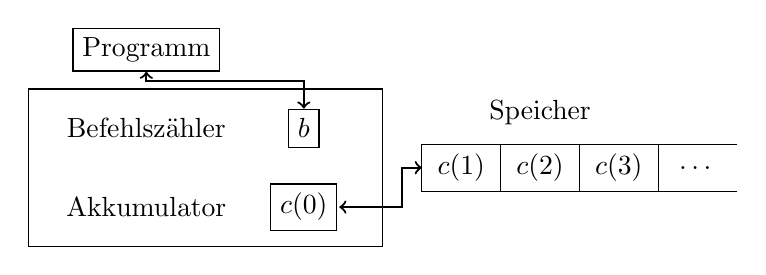
\begin{tikzpicture}
\node[draw] at (0,0) {Programm};
\node at (0,-1) {Befehlszähler};
\node[draw] at (2,-1) {$b$};
\node at (0,-2) {Akkumulator};
\node at (5,-0.8) {Speicher};
\node[draw] at (2,-2) {$c(0)$};
\draw (3.5,-1.8) rectangle (4.5,-1.2);
\node at (4,-1.5) {$c(1)$};
\draw (4.5,-1.8) rectangle (5.5,-1.2);
\node at (5,-1.5) {$c(2)$};
\draw (5.5,-1.8) rectangle (6.5,-1.2);
\node at (6,-1.5) {$c(3)$};
\draw (6.5,-1.8) -- (7.5,-1.8);
\node at (7,-1.5) {\ldots};
\draw (6.5,-1.2) -- (7.5,-1.2);
\draw (-1.5,-2.5) rectangle (3,-0.5);
\draw[<->,thick] (0,-0.28) -- (0,-0.4) -- (2,-0.4) -- (2,-0.75);
\draw[<->,thick] (2.45,-2) -- (3.25,-2) -- (3.25,-1.5) -- (3.5,-1.5);
\end{tikzpicture}
\end{center}
\end{figure}
\end{block}
 %TODO RAM
\end{frame}

\subsection{Turingmaschine}
\begin{frame}
\frametitle{Turingmaschine}
Eine Registermaschine ist zwar physikalischen Rechnern ähnlich, aber unhandlich um damit Beweise zu führen.
Daher ist ein abstrakteres Modell hilfreich \\
$\rightarrow$ Turingmaschine.
\pause
\begin{block}{Turingmaschine}
Die Turingmaschine besteht aus einem beidseitig \emph{unendlichen} Eingabe- und Rechenband
mit einem freibeweglichen Lese-/Schreibkopf, der von einer \emph{endlichen} Kontrolle gesteuert wird. 
\end{block}
\end{frame}
\begin{frame}
\vspace{-1cm}
\begin{block}{Definiton}
Eine Turingmaschine wird definiert als:
 \begin{itemize}
 \item $Q$, eine endliche Zustandsmenge
 \item $\Sigma$, einem endlichen Eingabealphabet
 \item $\sqcup$, einem Blanksymbol mit $\sqcup \notin \Sigma$
 \item $\Gamma$, einem endlichen Bandalphabet mit $\Sigma \cup\{\sqcup\} \subseteq \Gamma$
 \item $s \in Q$, einem Startzustand
 \item $\delta: Q\times\Gamma \rightarrow Q\times\Gamma\times\{L, R, N\}$
 \item $F \subseteq Q$, einer Menge an Endzuständen
 \end{itemize}
\end{block}
\begin{block}{Bemerkung}
 Für $q\in F$ gilt: $\forall a \in \Gamma: \delta(q, a) = (q, a, N)$, d.h. die Berechnung der Turingmaschine stoppt.
\end{block}
\end{frame}

\frame{
	\frametitle{Graph einer Turingmaschine}
	\begin{center}
	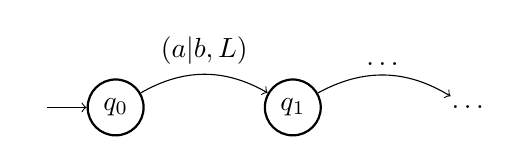
\begin{tikzpicture}[node distance=2.25cm,auto]
	\node(q0)[draw,circle,thick]{$q_0$};
	\node (s) [node distance=1cm,left of =q0]{};
	\node(q1)[draw,circle,thick,right of=q0]{$q_1$};
	\node(qx)[right of=q1]{\dots};

	\path[->]       (s) edge (q0)
	                (q0) edge[bend left] node{$(a|b,L)$} (q1)
			                (q1) edge[bend left] node{\dots} (qx);
					\end{tikzpicture}
					\end{center}

					Dabei steht die Kantenbeschriftung ``$(a|b,L)$'' für den Übergang $\delta(q_0,a) =
					(q_1,b,L)$.

					\vspace{2mm}
					Falls es für einen gegebenen Zustand und ein gegebenes
					Symbol keinen Zustandsübergang gibt, bricht die Maschine die Berechnung ab. 
}


\begin{frame}
\frametitle{Turingmaschine}
 \label{sec:busy_beaver}

Konstruieren Sie eine Turingmaschine, die aus drei Zuständen (plus einem
weiteren Haltezustand $q_f$) besteht und folgendes Verhalten hat:
\begin{quote}
  Angesetzt auf ein leeres Band schreibt sie möglichst viele ${\tt 1}$
  hintereinander und \textbf{hält} nach endlich vielen Schritten.
\end{quote}
Die Turingmaschine soll folgende Alphabete verwenden: $\Sigma = \{{\tt 1}\},
\Gamma = \Sigma \cup \{{\tt 0}\}$.  Insbesondere ist also ${\tt 0}$ das
Blanksymbol.

Welche Konfigurationen durchläuft die Maschine, wenn Sie auf dem leeren Band
gestartet wird?  Welche Konfigurationen durchläuft die Maschine bei Eingabe
des Wortes {\tt 101}?
\end{frame}
\begin{frame}
 Geben Sie eine wohldokumentierte Turingmaschine an, die zwei durch Blank
getrennte Binärworte aus $\{0,1\}^*$ addiert.
\end{frame}

\subsection{Entscheidbarkeit}
\begin{frame}
 \frametitle{Definitionen zur TM (Vorlesung)}
 \begin{enumerate}
  \item Eine TM \emph{akzeptiert} eine Eingabe $w \in \Sigma^*$, wenn sie nach Lesen von $w$ in einem Zustand aus $F$ stoppt.
  \item Sie \emph{akzeptiert} eine Sprache $L \subseteq \Sigma^*$ genau dann, wenn sie ausschließlich Wörter $w$ aus $L$ als Eingabe akzeptiert.
  \item Eine Sprache $L \subseteq \Sigma^*$ heißt \emph{rekursiv} oder \emph{entscheidbar}, wenn es eine Turingmaschine gibt, die auf allen Eingaben stoppt und
	ein Wort $w \in \Sigma^*$ genau dann akzeptiert, wenn $w \in L$ gilt.
  \item Eine Sprache $L \subseteq \Sigma^*$ heißt \emph{rekursiv-aufzählbar} oder \emph{semi-entscheidbar}, wenn es eine Turingmaschine gibt, 
	die genau $w$ genau dann akzeptiert, wenn $w \in L$ gilt. Das Verhalten der Turingmaschine für Eingaben $w \not\in L$ ist damit nicht definiert.
	Sie stoppt entweder nicht in einem Endzustand oder aber stoppt garnicht.
 \end{enumerate}
\end{frame}

\begin{frame}
 \frametitle{Beispiel zur Akzeptanz}
 \begin{itemize}
  \item $\Sigma := \{a, b\}$  
  \item $F := \{q_4\}$
 \end{itemize}
\vspace{-2cm}
 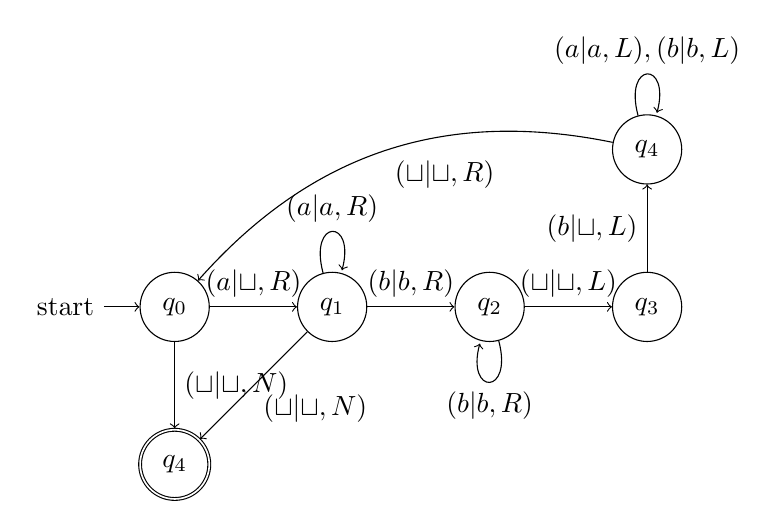
\begin{tikzpicture}[node distance=2cm,auto]
  \node(q0)[state,initial]{$q_0$};
  \node(q1)[state,right of=q0]{$q_1$};
  \node(q2)[state,right of=q1]{$q_2$};
  \node(q3)[state,right of=q2]{$q_3$};
  \node(q4)[state,above of=q3]{$q_4$};
  \node(q5)[state,accepting,below of=q0]{$q_4$};
  \path[->]       (q0) edge node{$(a|\sqcup,R)$} (q1)
	          (q0) edge node{$(\sqcup|\sqcup,N)$} (q5)
	          (q1) edge[loop above] node{$(a|a,R)$} ()
	          (q1) edge node{$(b|b,R)$} (q2)
	          (q1) edge node{$(\sqcup|\sqcup,N)$} (q5)
	          (q2) edge[loop below] node{$(b|b,R)$} ()
	          (q2) edge node{$(\sqcup|\sqcup,L)$} (q3)
	          (q3) edge node{$(b|\sqcup,L)$} (q4)
	          (q4) edge[loop above] node{$(a|a,L), (b|b,L)$} ()
	          (q4) edge[bend right] node{$(\sqcup|\sqcup,R)$} (q0);
 \end{tikzpicture}
 \end{frame}

\begin{frame}
 \frametitle{Sprache}
 \begin{itemize}
  \item $aab$ wird von der TM akzeptiert.
  \item $abb$ nicht.
  \item Die akzeptierte Sprache ist $L(TM) := \{a^kb^l| k >= l\}$
  \item Die Sprache ist offensichtlich semi-entscheidbar.
  \item Ist sie auch entscheidbar?
 \end{itemize}
\end{frame}


%TODO Beispiel für nicht entscheidbare Probleme
%TODO Beispiel für Entscheidbarkeit

\subsection{Universelle Turingmaschine}
\begin{frame}
\frametitle{Universelle Turingmaschine}
\begin{block}{Gödelnummer}
Jede Turingmaschine lässt sich eindeutig als Zahl kodieren. Eine solche Kodierung einer Turingmaschine nennen wir eine Gödelnummer dieser Turingmaschine. Wir vereinbaren weiterhin, dass alle gemäß unserer Kodierung ungültigen Gödelnummern einer TM zugeordnet werden, die alle Eingaben ablehnt.
\end{block}
\begin{block}{Universelle Turingmaschine}
Es existieren Turingmaschinen, die jede andere Turingmaschine bei Angabe der Entsprechenden Gödelnummer (also einer Kodierung), simulieren können. Diese TM erhält als Eingabe die Kodierung einer TM sowie eine Eingabe für die zu simulierende TM, und gibt die Ausgabe der simulierten TM aus.
\end{block}
\end{frame}

\begin{frame}
 \frametitle{Nicht entscheidbare Sprache}
 \begin{block}{Beispiel}
 \begin{itemize}
  \item Die Sprache aller ``Busy-Beaver''-Turingmaschinen mit 15 Zuständen ist nicht entscheidbar.
  \item Warum nicht?
 \end{itemize}
 \end{block}
\end{frame}

\begin{frame}
\frametitle{Aufgaben zur Entscheidbarkeit}
 Seien $L_1$ und $L_2$ zwei Sprachen über einem Alphabet $\Sigma$.
Beweisen Sie:
\begin{enumerate}
\item Ist $L_1$ entscheidbar, so ist auch $L_1^c$ entscheidbar.
\item Sind $L_1$ und $L_2$ entscheidbar, so ist auch $L_1\cup L_2$ entscheidbar.
\item Sind $L_1$ und $L_2$ entscheidbar, so ist auch $L_1\backslash L_2$ entscheidbar.
\item Ist $L_1$ entscheidbar, so ist auch die Sprache 
$$\min(L_1):=\{x\in L_1\mid \text{kein echtes Präfix von $x$ ist in }L_1 \}$$
entscheidbar.
\end{enumerate}
\end{frame}

\begin{frame}
 \frametitle{Aufgabe zur Semi-Entscheidbarkeit}
Sei $L$ eine semi-entscheidbare Sprache, die nicht entscheidbar ist. Ist die
Sprache $L'=\{0w:w \in L\} \cup \{1w: w \not\in L\}$ entscheidbar,
semi-entscheidbar oder keins von beiden?

Hinweis: Nimm an, $L'$ sei semi-entscheidbar, und folgere daraus, dass
dann $L$ entscheidbar ist. 
\end{frame}


\begin{frame}
 \frametitle{Halteproblem}
 Zeigen Sie, dass das Halteproblem semi-entscheidbar ist.
\end{frame}

\subsection{Erweiterungen von Turingmaschinen}
\begin{frame}
\frametitle{Erweiterungen von Turingmaschinen}
\begin{block}{Erweiterungen}
Es gibt mehrere, zu Turingmaschinen (bzgl. Berechenbarkeit) äquivalente Berechnungsmodelle, die der Turingmaschine sehr ähnlich sind. Man spricht hier von Erweiterungen von Turingmaschinen. Diese verwendet man gerne in z.B. Beweisen, da sie oft Übersichtlicher sind.
\end{block}
\end{frame}
% Mehrkopf
\begin{frame}
\frametitle{Mehrkopf-Turingmaschinen}
\vspace{-2cm}
\begin{figure}[H]
\begin{center}
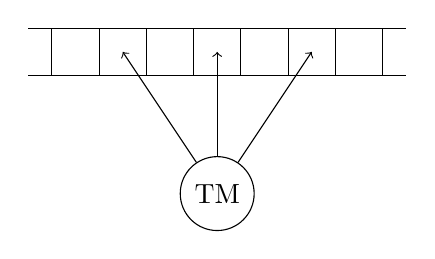
\begin{tikzpicture}[scale=0.3]
\draw (-8,1) -- (8,1);
\draw (-8,-1) -- (8,-1);
\draw (7,1) -- (7,-1);
\draw (5,1) -- (5,-1);
\draw (3,1) -- (3,-1);
\draw (1,1) -- (1,-1);
\draw (-1,1) -- (-1,-1);
\draw (-3,1) -- (-3,-1);
\draw (-5,1) -- (-5,-1);
\draw (-7,1) -- (-7,-1);
\node[draw,circle] (tm) at (0,-6) {TM};
\draw[->] (tm) -- (0,0);
\draw[->,bend left] (tm) -- (-4,0);
\draw[->,bend right] (tm) -- (4,0);
\end{tikzpicture}
\end{center}
\end{figure}
Eine Mehrkopf-Turingmaschine hat mehrere Lese-/Schreibeköpfe. Die Zustandsänderung hängt nun von dem gelesenen Zeichen aller Köpfe ab und kann auch alle Köpfe verschieben bzw. mit allen gleichzeitig schreiben.
\begin{block}{Änderungen in der Definition}
$$ \delta: Q \times \Gamma^n \rightarrow Q \times \Gamma^n \times \{L,N,R\}^n$$
\end{block}
\end{frame}

% Mehrband
\begin{frame}
\frametitle{Mehrband-Turingmaschinen}
\vspace{-2cm}
\begin{figure}[H]
\begin{center}
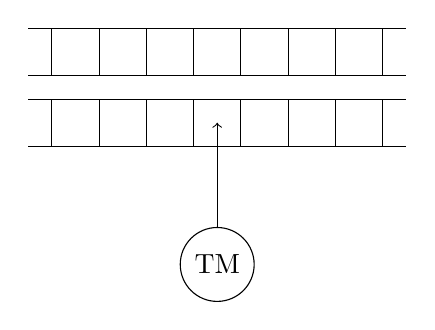
\begin{tikzpicture}[scale=0.3]
\draw (-8,4) -- (8,4);
\draw (-8,2) -- (8,2);
\draw (7,4) -- (7,2);
\draw (5,4) -- (5,2);
\draw (3,4) -- (3,2);
\draw (1,4) -- (1,2);
\draw (-1,4) -- (-1,2);
\draw (-3,4) -- (-3,2);
\draw (-5,4) -- (-5,2);
\draw (-7,4) -- (-7,2);

\draw (-8,1) -- (8,1);
\draw (-8,-1) -- (8,-1);
\draw (7,1) -- (7,-1);
\draw (5,1) -- (5,-1);
\draw (3,1) -- (3,-1);
\draw (1,1) -- (1,-1);
\draw (-1,1) -- (-1,-1);
\draw (-3,1) -- (-3,-1);
\draw (-5,1) -- (-5,-1);
\draw (-7,1) -- (-7,-1);

\draw (-8,1) -- (8,1);
\draw (-8,-1) -- (8,-1);
\draw (7,1) -- (7,-1);
\draw (5,1) -- (5,-1);
\draw (3,1) -- (3,-1);
\draw (1,1) -- (1,-1);
\draw (-1,1) -- (-1,-1);
\draw (-3,1) -- (-3,-1);
\draw (-5,1) -- (-5,-1);
\draw (-7,1) -- (-7,-1);
\node[draw,circle] (tm) at (0,-6) {TM};
\draw[->] (tm) -- (0,0);
\end{tikzpicture}
\end{center}
\end{figure}
Eine Mehrband-Turingmaschine hat mehrere Bänder. Die Zustandsänderung kann nun auch auf ein anderes Band wechseln. Dabei wird immer auf die zuletzt eingenommene Position auf dem anderen Band gewechselt 
\begin{block}{Änderungen in der Definition}
$$ \delta: Q \times \Gamma \times \{1, \ldots, n\} \rightarrow Q \times \Gamma \times \{L,N,R\} \times \{1, \ldots, n\}$$
\end{block}
\end{frame}
% Mehrdim
\begin{frame}
\frametitle{Mehrkopf Turingmaschinen}
\vspace{-2cm}
\begin{figure}[H]
\begin{center}
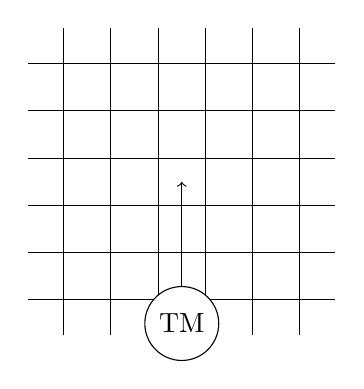
\begin{tikzpicture}[scale=0.3]
\draw[step=2cm,xshift=1cm,yshift=1cm] (-7.5,-7.5) grid (5.5,5.5);
\node[draw,circle,fill=white] (tm) at (0,-6) {TM};
\draw[->] (tm) -- (0,0);
\end{tikzpicture}
\end{center}
\end{figure}
Eine Mehrdimensionale Turingmaschine hat ein Mehrdimensionales Band, der Kopf kann sich dann in allen verfügbaren Dimensionen bewegen.
\begin{block}{Änderungen in der Definition (für Dimension 2)}
$$ \delta: Q \times \Gamma \rightarrow Q \times \Gamma \times \{L,N,R,U,D\}$$
\end{block}
\end{frame}

% Beispiel (if time)
% Aufgabe
\begin{frame}
\frametitle{Aufgabe}
\vspace{-1cm}
Eine $k$-Band-Turingmaschine ist eine Turingmaschine mit $k$
Arbeitsbändern und der Übergangsfunktion

\[ \delta: Q \times \Gamma \times \{1, \ldots, k\} \to
Q \times \Gamma \times \{L, R, N\} \times \{1, \ldots, k\}, \]

wobei $\delta(q, a, i) = (p, b, X, j)$ bedeute:

\begin{quote}
  Wenn sich die Maschine im Zustand $q$ befindet und
  auf Band $i$ das Symbol $a$ liest, so springt die Maschine in Zustand $p$,
  überschreibt $a$ mit $b$, der Lese-Schreib-Kopf bewegt sich auf Band $i$
  gemäß $X$ und springt auf Band $j$ an die Stelle, an der er sich
  auf diesem Band zuletzt befunden hat.
\end{quote}

Die Eingabe befinde sich auf Band 1, und im Zustand $s$ befinde sich der
Kopf an der ersten Stelle der Eingabe. Die Stelle, auf die der Kopf bei einem
Wechsel auf ein bis dahin unbenutztes Band springt, sei
festgelegt.
Eine solche 2-Band-Turingmaschine habe nun Zeitaufwand $T(n)$.
Zeigen Sie informell, dass diese von einer einfachen
Turingmaschine mit Zeitaufwand $O(T^2(n))$ simuliert werden kann.\\
\end{frame}

\subsection{Satz von Rice}
\begin{frame}
\frametitle{Satz von Rice}
Der Satz von Rice sagt aus, dass es unmöglich ist, eine nichttriviale Eigenschaft von Turingmaschinen algorithmisch zu entscheiden.
\begin{block}{Formale Version}
Es sei R die Klasse aller Turing-berechenbaren Funktionen und $S$ eine beliebige nichttriviale (das bedeutet $S \neq \emptyset$ und $S \neq R$) Teilmenge davon. Dann ist die Sprache
$$ C_S = \{ i |\text{ die von $M_i$ berechnete Funktion liegt in $S$} \} $$
Unentscheidbar. 
\end{block}
\end{frame}
% Beispiel
\begin{frame}
\frametitle{Beispiel}
Die Klasse aller Programme die etwas auf einem Rechner tun, das der Benutzer nicht möchte (das ist eine Teilmenge der Turingberechenbaren Funktionen) ist unentscheidbar. Daraus folgt, dass es keinen perfekten Virenscanner geben kann!
\end{frame}

% Aufgabe
\begin{frame}
\frametitle{Aufgabe}
Kann man die Entscheidbarkeit der folgenden Mengen mithilfe des Satzes von Rice bestimmen?
\begin{itemize}
\item Alle Turingmaschinen die nur $0$ aufs Band Schreiben.
\item Alle Turingmaschinen die im ersten Schritt genau eine $0$ aufs Band Schreiben und im zweiten Schritt anhalten. 
\item Alle Turingmaschinen die überhaupt etwas auf das Band schreiben.
\end{itemize}
\end{frame}

\subsection{Postsches Korrespondenzproblem}
\begin{frame}
\frametitle{Postsches Korrespondenzproblem}
Gegeben sei einer Folge von Paaren $((x_1, y_1), (x_2, y_2), \ldots, (x_n,y_n))$ von nichtleeren Worten über einem endlichen Alphabet. Dies nennt man eine \textbf{Instanz} des PKP.
Eine nicht-leere Folge $I = i_1, i_2, \ldots, i_m$ von indices $\{1, \ldots, n\}$ heißt Lösung zu $P$, wenn $x_{i_1}x_{i_2}\ldots{}x_{i_m} = y_{i_1}y_{i_2}\ldots{}y_{i_m}$.
\begin{block}{Beispiel}
\begin{displaymath}
\{ {a \choose aba}, {ab \choose bb}, {baa \choose aa} \}
\end{displaymath}

Lösung: $1,3,2,3$
\begin{displaymath}
{a \choose aba}, {baa \choose aa}, {ab \choose bb}, {baa \choose aa}
\end{displaymath}

\end{block}
\end{frame}

\begin{frame}
\frametitle{Aufgabe}
\begin{enumerate}
\item Finde eine Lösung für folgende Instanz des Post'schen Korrespondenzproblems: 
\[ ((aa, a), (b, aa), (a, aab)) \]
  \item Zeigen Sie, dass folgende Instanz des Post'schen Korrespondenzproblems
        keine Lösung hat:

        \[ ((ab, b), (bba, abb), (ab, ba), (a, abb)) \]

  \item Zeigen Sie, dass das Post'sche Korrespondenzproblem für Wörter
über einem Alphabet mit nur einem Symbol entscheidbar ist.
\end{enumerate}
\end{frame}

\begin{frame}
\frametitle{Aufgabe}
Finde eine Lösung für folgendes PCP
$$ ((001,0),(01,011),(01,101),(10,001)) $$
\pause
Eine kürzeste Lösung hat mindestens die Länge 66, z.B:
\begin{center}
$ I_1 = $(2,4,3,4,4,2,1,2,4,3,4,3,4,4,3,4,4,2,1,4,\\
4,2,1,3,4,1,1,3,4,4,4,2,1,2,1,1,1,3,4,3,4,1,2,\\
1,4,4,2,1,4,1,1,3,4,1,1,3,1,1,3,1,2,1,4,1,1,3)
\end{center}
\end{frame}

\section{Probleme}
\begin{frame}
 \frametitle{Probleme}
 \begin{block}{Definition (Skript)}
 Ein \emph{Problem $\Pi$} ist gegeben durch:
 \begin{enumerate}
  \item eine allgemeine Beschreibung aller vorkommenden Parameter;
  \item eine genaue Beschreibung der Eigenschaften, welche die Lösung haben soll
 \end{enumerate}
 \end{block}
 Ein \emph{Problembeispiel} \textit{I} \emph{(Instanz)} von $\Pi$ erhalten wir, indem wir die Parameter von $\Pi$ festlegen.
\end{frame}

\begin{frame}
 \frametitle{Entscheidungsproblem}
 \begin{block}{Definition}
  Ein Entscheidungsproblem ist ein Problem, bei dem die Lösung aus ``Ja'' oder ``Nein'' besteht. 
  Entscheidungsprobleme lassen sich gut auf Sprachen abbilden.
 \end{block}
\end{frame}

\begin{frame}
 \frametitle{Optimierungsproblem und Entscheidungsproblem}
 \begin{block}{Beispiel}
  \begin{enumerate}
   \item Die Aufgabe, aus einem gegebenen Blech möglichst viele sternförmige Weihnachtsplätzchen zu gewinnen, ist ein Optimierungsproblem.
   \item Die Frage, ob aus diesem Blech mindestens k Plätzchen gewonnen werden können, ist ein zugehöriges Entscheidungsproblem.
  \end{enumerate}
 \end{block}
 \begin{block}{Überlegung}
  Wie kann man mit einer Turingmaschine, welche das Entscheidungsproblem löst, das Optimierungsproblem lösen?
 \end{block}
 Hinweis: Nimm an, dass es nur endlich viele mögliche Kekskonfigurationen auf einem Backblech gibt.
\end{frame}

\begin{frame}
 \begin{block}{Überlegung}
  Wie kann man mit einer Turingmaschine, welche das Entscheidungsproblem löst, das Optimierungsproblem lösen?
 \end{block}
\begin{block}{Strategie}
 \begin{enumerate}
  \item Zunächst mit binärer Suche das maximale k herausfinden.
  \item Eine Formplatzierung festlegen, danach vorherigen Schritt wiederholen. Wenn sich das k gesenkt hat, war die Platzierung falsch. 
  Wenn nicht, war sie richtig
  \item Wiederhole bis alle Formen platziert sind.
 \end{enumerate}
\end{block}
\end{frame}


%TODO: Grafik

\begin{frame}
 \frametitle{Entscheidungsproblem}
 \begin{block}{TUT}
  Gegeben seien eine Tutoriumsliste mit m Tutorien und Tutoriumswahlen von n Studenten. Jedes Tutorium kann nur l Teilnehmer haben.
 Das Entscheidungsproblem \textit{TUT} besteht darin, zu entscheiden, ob alle Studenten ihr Wunschtutorium bekommen können.
 \end{block}
 \begin{itemize}
  \item Kann man aus diesem Entscheidungsproblem ähnliche Entscheidungsprobleme konstruieren?
  \item Formuliere das zugehörige Optimierungsproblem.
 \end{itemize}
\end{frame}

\begin{frame}
 \begin{block}{Ähnliche Entscheidungsprobleme}
  \textit{TUT-k}: Können mindestens k Studenten ihr Wunschtutorium bekommen.
  Lässt sich für $0 \leq k \leq n$ formulieren.
 \end{block}
 \begin{block}{Optimierungsproblem}
  Finde die Belegung, welche die Anzahl der gewählten Zuteilungen maximiert.
 \end{block}
\end{frame}

\begin{frame}
 \frametitle{Optimierungsproblem}
 Gegeben sei ein Graph $G=(V,E)$ mit $V:=\{1,\ldots,n\}$ und $E\subseteq \{\{u,v\} \mid u,v \in V, u\neq v\}$. Weiter seien $c:E \rightarrow \mathbb{R}^+$ eine Längenfunktion auf den Kanten des Graphen sowie $s\in V$ ein ausgewiesener Start- und $t\in V$ ein ausgewiesener Zielknoten. 
Ein Pfad von $s$ nach $t$ ist eine Folge von Kanten $p = \{i_1,i_2\},\{i_2,i_3\},\ldots,\{i_{k-2},i_{k-1}\},\{i_{k-1},i_k\}$ mit $\{i_j, i_{j+1}\} \in E$ und $i_1=s$ sowie $i_k=t$. 
Die Länge des Pfades sei definiert als die Summe der Längen aller Kanten auf dem Pfad. 
Betrachten Sie die Menge der Pfade, die von $s$ nach $t$ führen, und formulieren Sie ein naheliegendes Optimierungsproblem. 
Formulieren Sie ein zu Ihrem Optimierungsproblem gehörendes Entscheidungsproblem.
\end{frame}

\subsection{Kodierungsschemata}
\begin{frame}
 \frametitle{Kodierungsschemata (VL)}
 \begin{block}{Definition Kodierungsschema}
 Ein \emph{Kodierungsschema} s ordnet jedem Problembeispiel eines Problems eine Zeichenkette oder Kodierung über einem Alphabet $\Sigma$ zu. 
 Die Inputlänge eines Problembeispiels ist die Anzahl der Symbole seiner Kodierung.
 Dabei gibt es natürliche verschiedene Kodierungsschemata für ein bestimmtes Problem.
 \end{block}
 \begin{block}{Äquivalenz}
  Zwei Kodierungsschemata $s_1$, $s_2$ heißen \emph{äquivalent} bezüglich eines Problems $\Pi$, falls es Polynome p1, p2 gibt, so dass gilt:
  \[
   (|s_1(I)| = n \Rightarrow |s_2(I)| \leq p_2(n))\mbox{ und } (|s_2(I)| = m \Rightarrow |s_1(I)| \leq p_1(m))
  \]
für alle Problembeispiele I von $\Pi$.
 \end{block}
\end{frame}

\begin{frame}
 \frametitle{Kodierungsschemata}
 Das Entscheidungsproblem \textit{PRIMES} besteht darin, zu entscheiden, ob es sich bei einer gegebenen natürlichen Zahl $p>1$ um eine Primzahl handelt. 
Eine Probleminstanz von \textit{PRIMES} wird also durch eine natürliche Zahl kodiert. 
Für $b\in \mathbb{N}$ bezeichne $s_b$ das Kodierungsschema, welches Zahlen zur Basis $b$ darstellt.

Zeigen Sie, dass die Kodierungsschemata $s_a$ und $s_b$ für $a,b>1$ bezüglich \textit{PRIMES} äquivalent sind.

\begin{block}{Überlegung}
 Welches Kodierungsschema c wäre zu a, b nicht äquivalent? Warum nicht?
\end{block}
\end{frame}

\begin{frame}
\frametitle{Kodierung von TUT}
 \begin{block}{Wiederholung: TUT}
  Gegeben seien eine Tutoriumsliste mit m Tutorien und Tutoriumswahlen von n Studenten. Jedes Tutorium kann nur l Teilnehmer haben.
 Das Entscheidungsproblem \textit{TUT} besteht darin, zu entscheiden, ob alle Studenten ihr Wunschtutorium bekommen können.
 \end{block}
 \begin{block}{Überlegung}
 Wie sähe ein mögliches Kodierungsschema auf dem Alphabet $\Sigma = \{0,1,\#\}$ aus?
 \end{block}
 \pause
 \begin{block}{Mögliche Kodierung}
 $m\#n\#l$ gefolgt von $\#i\#j \mbox{ für } 1 \leq i \leq n$, falls Teilnehmer i Tutorium j gewählt hat.
 \end{block}
\end{frame}

\begin{frame}
\frametitle{Kodierung von TUT}
\begin{block}{Beispiel}
 Gegeben sei eine Instanz \textit{I} von TUT mit 2 Tutorien, 5 Studenten, einer maximalen Teilnehmerzahl von 3 und folgenden Wahlen:
 \begin{enumerate}
  \item Student 1 wählt Tutorium 2
  \item Student 2 wählt Tutorium 2
  \item Student 3 wählt Tutorium 1
  \item Student 4 wählt Tutorium 2
  \item Student 5 wählt Tutorium 2
 \end{enumerate}
\end{block}
\pause
\begin{block}{Kodierung}
$10\#101\#11 \#001\#010 \#010\#010 \#011\#001 \#100\#010 \#101\#010$
\end{block}
\end{frame}

\begin{frame}
\frametitle{TUT}
\begin{block}{Beispiel}
 Gegeben sei eine Instanz \textit{I} von TUT mit 2 Tutorien, 5 Studenten, einer maximalen Teilnehmerzahl von 3 und folgenden Wahlen:
 \begin{enumerate}
  \item Student 1 wählt Tutorium 2
  \item Student 2 wählt Tutorium 2
  \item Student 3 wählt Tutorium 1
  \item Student 4 wählt Tutorium 2
  \item Student 5 wählt Tutorium 2
 \end{enumerate}
\end{block}
\begin{block}{Optimierungsproblem}
 Was ist hier eine Lösung des Optimierungsproblems? 
\end{block}
\end{frame}

\subsection{Die Klasse P}
\begin{frame}
\frametitle{Die Klasse $\mathcal{P}$}
Die Klasse $\mathcal{P}$ ist definiert als die Menge aller Sprachen, die von einer (deterministischen) Turingmaschine, deren Zeitkomplexität höchstens polynomial ist, entschieden werden können.\\[6pt]
\end{frame}

\begin{frame}
\frametitle{Beispiel}
\textbf{Anmerkung:} Da eine RAM Maschine in Polyzeit von einer TM simuliert werden kann, kann man (auf einer abstrakteren Ebene) i.A. Komplexitäten von bekannten Algorithmen in Beweisen verwenden.\\[10pt]
Die folgende Sprache ist in $\mathcal{P}$: Die gerichteten Graphen zusammen mit einem Start- und einem Endknoten, so dass der Endknoten vom Startknoten aus über die Kanten erreichbar ist.\\[6pt]
\textbf{Grober Beweis:}	Tiefensuche ist in $\mathcal{O}(|\mathcal{V}| + |\mathcal{E}|)$
\end{frame}

\begin{frame}
\frametitle{Sind folgende Sprachen in $\mathcal{P}$?}
\begin{itemize}
\item Die Wörter der deutschen Sprache
\item Die ungraden Zahlen
\item Eine reguläre Sprache $L$
\item Die PCPs die eine Lösung haben
\item Die unär kodierten Primzahlen
\item Die binär kodierten Primzahlen
\end{itemize}
\end{frame}

\begin{frame}
 \frametitle{Laufzeitbetrachtung}
 Betrachten Sie $L_1 := L[\text{\textit{PRIMES}},s_1]$. 
Ein naiver Algorithmus für \textit{PRIMES} könnte alle Zahlen $2,3,\ldots,p-1$ darauf hin überprüfen, ob sie die gegebene Zahl $p$ teilen. 
Beschreiben Sie kurz in Worten die Arbeitsweise einer \textbf{deterministischen} Turing-Maschine, die diesen Algorithmus implementiert und damit $L_1$ entscheidet. 
Geben Sie die Laufzeit Ihrer Turing-Maschine asymptotisch an. Ist $L_1$ in $\mathcal{P}$? Begründen Sie gegebenenfalls, warum $L_1$ in $\mathcal{P}$ ist.
\end{frame}

\subsection{Nichtdeterministische Turingmaschinen}
\begin{frame}
\frametitle{Nichtdeterministische Turingmaschinen}

\begin{block}{Version aus der Vorlesung}
Wir definieren eine nichtdeterministische Turingmaschine als Erweiterung einer deterministischen.
 Wir erweiteren die TM um ein \emph{Orakelmodul}, das bevor der deterministischen Berechnung Zeichen auf das Band links von der Eingabe schreibt,
 danach verfährt die Maschine wie eine normale TM.
 Die NDTM akzeptiert genau die Wörter, für die es eine Ausgabe des Orakelmoduls gibt,
 sodass der deterministische Anteil der Machine das Wort akzeptiert.
\end{block}
\end{frame}
\begin{frame}
\frametitle{Nichtdeterministische Turingmaschinen: Anmerkung}
Es gibt weitere dazu äquivalente Definitionen von NDTMs:
 Man kann auch analog zu nichtdeterministischen endlichen Automaten, die NDTM als normale Turingmaschinen mit nicht eindeutiger Übergangsfunktion definieren,
 diese akzeptiert dann ebenfalls analog wenn ein akzeptierender Pfad existiert.\\
\end{frame}
% NP als Klasse

\subsection{Die Klasse NP}
\begin{frame}
\frametitle{$\mathcal{NP}$}
\begin{block}{$\mathcal{NP}$}

$\mathcal{NP}$ ist (analog zu $\mathcal{P}$) die Klasse aller Sprachen die von einer nichtdeterministischen Turingmaschine in Polyzeit erkannt werden.
\end{block}\vspace{1cm}
\textbf{Anmerkung}: Die Frage ob $\mathcal{P} = \mathcal{NP}$ oder nicht ist ein großes, offenes Problem.
\end{frame}

\begin{frame}
\frametitle{Grundidee: $\mathcal{NP}$-Entscheider}
Üblicherweise geht eine TM die ein Problem aus $\mathcal{NP}$ entscheidet folgendermaßen vor: 
\begin{enumerate}
\item Rate Sogenannten "Zeugen" für $x \in L$ (Nichtdeterministisch)
\item Überprüfe ob Zeuge korrekt. (in Polyzeit)
\item Falls ja, halte mit Ausgabe $x \in L$
\end{enumerate}
Man spricht daher auch von den \emph{effizient verifizierbaren} Entscheidungsproblemen.
\end{frame}

\begin{frame}
\frametitle{$\mathcal{NP}$}
 Betrachten Sie die Sprache $L_{10}^c := L[\text{\textit{PRIMES}},s_{10}]^c$ der \textit{zusammengesetzten} Zahlen in Dezimaldarstellung. 
Beschreiben Sie grob in Worten die Arbeitsweise einer \textbf{nichtdeterministischen} Turing-Maschine, die $L_{10}^c$ entscheidet. 
Ein Unterprogramm für die Division von Dezimalzahlen mit polynomieller Laufzeit sei gegeben und kann von Ihrer Turing-Maschine aufgerufen werden. 
Ist $L_{10}^c$ in $\mathcal{NP}$? Begründen Sie gegebenenfalls, warum $L_{10}^c$ in $\mathcal{NP}$ ist.

\medskip
\textit{Hinweis:} Überlegen Sie sich, was Ihre Turing-Maschine in der Orakel-Phase sinnvollerweise auf das Band schreiben könnte.
\end{frame}


% Unentscheidbarkeit universelle Sprache
\begin{frame}
\frametitle{Unentscheidbarkeit ohne Rice}
\begin{block}{Universelle Sprache (Vorlesung)}
Die Universelle Sprache ist definiert als: $L_u := \{wv | v \in L(T_w)\}$
\end{block}
Also: Die Menge aller Wörter $wv$ so dass $T_w$ das Wort $v$ akzeptiert und hält.
\end{frame}

\begin{frame}
\frametitle{Unentscheidbarkeit ohne Rice}
\begin{block}{Universelle Sprache (Vorlesung)}
Die Universelle Sprache ist definiert als: $L_u := \{wv | v \in L(T_w)\}$
\end{block}
\begin{block}{Erinnerung: Diagonalsprache}
Die Diagonalsprache $L_d$ ist definiert als: $L_d := \mathcal{M}_i$ akzeptiert $w_i$ nicht
\end{block}
Um zu zeigen, dass $L_u$ unentscheidbar ist, wollen wir wie folgt vorgehen: Wie nehmen an wir könnten $L_u$ entscheiden und zeigen, dass wir unter dieser Voraussetzung auch $L_d^c$ entscheiden können.
\begin{itemize}
\item Annahme: Es existierte eine TM $\mathcal{M}$, die $L_u$ Entscheiden kann.
\item Für eine Instanz aus $L_d^c$, berechne $w_i$ und übergebe $\mathcal{M}$ das Wort: $<M_i>w_i$
\item Gebe das Ergebnis von $\mathcal{M}$ aus
\end{itemize}
\end{frame}

\begin{frame}
\frametitle{Polyreduktionen}
\begin{block}{Definition (Vorlesung)}
Eine polynomielle Transformation einer Sprache $L_1$ in eine Sprache $L_2$ ist eine Funktion
$f: \Sigma^*_1 \rightarrow \Sigma^*_2$ mit den Eigenschaften:
\begin{enumerate}
\item Es existiert eine deterministische Turing-Maschine, die in polynomieller Zeit $f$ berechnet
\item für alle $x$ gilt: $x \in L_1 \iff f(x) \in  L_2$
\end{enumerate}
Wir schreiben dann $L_1 \propto L_2$ ($L_1$ ist polynomial transformierbar in (reduzierbar auf) $L_2$ ).
\end{block}
\textbf{Anmerkung}: In welche Richtung das $\propto$ Symbol zeigt kann man sich folgerndermaßen  merken:
$L_2$ ist das "schwerere" Problem. Kann man $L_2$ entscheiden, so kann man mit polynomiellen Aufwand auch $L_1$ entscheiden.
\end{frame}


% NP vollständigkeit
\subsection{NP-Vollständigkeit}
\begin{frame}
\frametitle{$\mathcal{NP}$-Schwere}
\begin{block}{$\mathcal{NP}$-Schwere}
Eine Sprache $L_1$ ist $\mathcal{NP}$-schwer gdw. 
\[\forall L_2 \in \mathcal{NP} \,\, : \,\, L_2 \propto L_1\]
\end{block}
\textbf{Anmerkung}: In diesem Sinne sind die $\mathcal{NP}$-schweren Probleme schwerer oder mindestens so schwer zu lösen wie alle Probleme in $\mathcal{NP}$.
\end{frame}

% Polyreduktion ist Transitiv, daher ist NPC cool
\begin{frame}
\frametitle{Transitivität von Polyreduktionen und $\mathcal{NP}$}
Polynomiale Transformationen sind transitiv, d.h. wenn $L_1 \propto L_2$ und $L_2 \propto L_3$ dann gilt auch $L_1 \propto L_3$.\\[8pt]
Ist $L_3 \in \mathcal{NP}$, so wissen wir, dass auch $L_1$ sowie $L_2 \in \mathcal{NP}$, man sprich auch davon, $L_1$ und $L_2$ auf $L_3$ polynomiell reduziert zu haben.\\[8pt]
Gegeben eine Sprache $L_N$, von der wir wissen das sie $\mathcal{NP}$-schwer ist, was wäre ein möglicher Ansatz um für eine weitere Sprache $L_X$ die $\mathcal{NP}$-Schwere zu beweisen?\\
\pause
Man zeigt $L_N \propto L_X$
\end{frame}

\begin{frame}
\frametitle{$\mathcal{NP}$-Vollständigkeit}
Eine Sprache $L$ ist $\mathcal{NP}$-vollständig genau dann, wenn
$$L \in \mathcal{NP}$$ sowie $$L\mbox{ ist $\mathcal{NP}$-schwer}$$
Damit sind die $\mathcal{NP}$-vollständigen Probleme, die ,,schwersten'' Probleme aus $\mathcal{NP}$.\\
Interessant ist $\mathcal{NP}$ vor allem, da man aus Aussagen über diese Probleme viel über alle Probleme aus $\mathcal{NP}$ aussagen kann.
Ist etwa $SAT \in \mathcal{P}$ so wäre $\mathcal{P} = \mathcal{NP}$. (warum?)
\end{frame}

\begin{frame}
\frametitle{CLIQUE}
\begin{block}{Problem}
\textbf{Gegeben:} Graph $G = (V, E)$ und ein Parameter $K \leq |V|$\\
\textbf{Problem:} Gibt es in G eine Clique der Größe mindestens $K$?
\end{block}
\begin{block}{Erinnerung}
Eine Clique ist ein vollständig verbundener Teilgraph, also eine Menge $V' \subseteq V$, so dass für alle $i,j \in V'$ mit $i\neq j$ gilt: $(i, j) \in E$.
\end{block}
\textit{Dieses Problem ist $\mathcal{NP}$-vollständig}
\end{frame}

\begin{frame}
\frametitle{CLIQUE Beispiel}
\vspace{-1cm}
\begin{figure}[H]
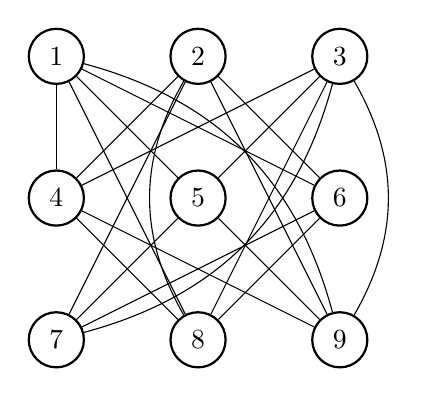
\begin{tikzpicture}[scale=1.8]
\tikzstyle{every node}=[circle, thick, minimum size = 7mm, draw]
\draw node (v1) at (0,2) {1};
\draw node (v2) at (1,2) {2};
\draw node (v3) at (2,2) {3};
\draw node (v4) at (0,1) {4};
\draw node (v5) at (1,1) {5};
\draw node (v6) at (2,1) {6};
\draw node (v7) at (0,0) {7};
\draw node (v8) at (1,0) {8};
\draw node (v9) at (2,0) {9};
\draw (v1) to (v4);
\draw (v1) to (v8);
\draw (v1) to [bend left] (v9);
\draw (v1) to (v5);
\draw (v1) to (v6);
\draw (v2) to (v4);
\draw (v2) to (v7);
\draw (v2) to [bend right] (v8);
\draw (v2) to (v9);
\draw (v2) to (v6);
\draw (v3) to (v4);
\draw (v3) to [bend left] (v7);
\draw (v3) to (v5);
\draw (v3) to (v8);
\draw (v3) to [bend left] (v9);
\draw (v4) to (v8);
\draw (v4) to (v9);
\draw (v5) to (v7);
\draw (v5) to (v9);
\draw (v6) to (v7);
\draw (v6) to (v8);
\end{tikzpicture}
\end{figure}
\begin{itemize}
\item Hat dieser Graph eine 3-CLIQUE?\pause
\item Hat dieser Graph eine 4-CLIQUE?
\end{itemize}
\end{frame}

\begin{frame}
\frametitle{$\mathcal{NP}$-Vollständigkeitsbeweis}
\begin{itemize}
 \item $CLIQUE \in \mathcal{NP}$: Übung\\
 \item $CLIQUE\mbox{ } \mathcal{NP}-schwer:$ Wir zeigen $3SAT \propto CLIQUE$. (warum?)\\\pause
 Wir müssen eine polynomielle Transformation einer $3SAT$-Instanz in eine $CLIQUE$-Instanz angeben. (warum?)\\
\end{itemize}
\end{frame}

\begin{frame}
\frametitle{$\mathcal{NP}$-Vollständigkeitsbeweis}
Sei $C = \{c_1, \ldots, c_n\}$ eine $3SAT$-Instanz mit 
$$ c_i = x_{i1} \vee x_{i2} \vee x_{i3} \mbox{ mit } x_{ij} \in \{u_1,\ldots,u_m,\bar{u_1},\ldots,\bar{u_m}\} $$
Konstruiere eine CLIQUE-Instanz $(G = (V, E), K)$ folgendermaßen:
$$V = (v_{1,1}, v_{1,2}, v_{1,3}, v_{2,1},\ldots,v_{n,1},v_{n,2},v_{n,3})$$
$$E = {(v_{i,j},v_{k,m})| (i \neq k \wedge x_{i,j} \neq \bar{x}_{k,m} )}$$%TODO Bar sucks, \lineover or smth?
$$K = n$$
\end{frame}

\begin{frame}
$$V = (v_{1,1}, v_{1,2}, v_{1,3}, v_{2,1},\ldots,v_{n,1},v_{n,2},v_{n,3})$$
Jeder Knoten steht also für ein Literal in der $3SAT$ Instanz. 
$$E = {(v_{i,j},v_{k,m})| (i \neq k \wedge x_{i,j} \neq \bar{x}_{k,m} )}$$%TODO Bar sucks, \lineover or smth?
Zwei Knoten sind verbunden, wenn sie gleichzeitig erfüllbar sind und nicht in der gleichen Klausel stehen. 
$$K = n$$
und wir suchen nach einer $CLIQUE$ der Größe $n$.\\
\end{frame}
\begin{frame}
\frametitle{$\mathcal{NP}$-Vollständigkeitsbeweis}
Wenn also eine $n-CLIQUE$ existiert, so heißt dies, wir haben $n$ erfüllbare Literale, die alle in jeweils unterschiedlichen Formeln stehen (Da ja alle untereinander verbunden sind). Das liefert uns eine erfüllende Wahrheitsbelegung. Eine $n$-$CLIQUE$ existiert also genau dann wenn es für die $3SAT$ Instanz eine erfüllende Wahrheitsbelegung gibt.\\
Da $CLIQUE$ $\mathcal{NP}$-schwer ist und in $\mathcal{NP}$ liegt, ist also $CLIQUE$ $\mathcal{NP}$-Vollständig.
\end{frame}

\begin{frame}
\frametitle{Allgemeines zu $NP$-Vollständigkeitsbeweise}
In der Regel ist es schwer zu zeigen, dass ein Problem $\mathcal{NP}$-schwer ist, aber leicht zu zeigen, dass ein Problem in $\mathcal{NP}$ liegt.\\[8pt]
Da man üblicherweise ein $\mathcal{NP}$-vollständiges Problem als Vorausetzung für die Reduktion benötigt (Ausnahme: Satz von Cook), lohnt es sich einige kennen zu lernen.
\end{frame}

\begin{frame}
\frametitle{SAT}
\begin{block}{Problem}
\textbf{Gegeben:}
\begin{itemize}
 \item Menge $U$ von Variablen
 \item Menge $C$ von Klauseln über $U$
\end{itemize}
\textbf{Frage:} Existiert eine erfüllende Wahrheitsbelegung von $C$?
\end{block}
\begin{itemize}
\item \emph{Das} Standardproblem.
\item Es gibt viele hochoptimierte "SAT-Solver". Steht man in der Praxis vor einem $\mathcal{NP}$-Problem, kann es sich anbieten die Transformation auf $SAT$ durchzuführen.
\end{itemize}
\end{frame}
\begin{frame}
\frametitle{3-SAT}
\begin{block}{Problem}
\textbf{Gegeben:}
\begin{itemize}
 \item Menge $U$ von Variablen
 \item Menge $C$ von Klauseln über $U$, jede Klausel enthält genau \emph{drei} Literale
\end{itemize}
\textbf{Frage:} Existiert eine erfüllende Wahrheitsbelegung von $C$?
\end{block}
\begin{itemize}
\item Bietet sich bei Reduktion eher an als $SAT$, da übersichtlicher
\end{itemize}
\end{frame}
\begin{frame}
\frametitle{MAX2SAT}
\begin{block}{Problem}
\textbf{Gegeben:}
\begin{itemize}
 \item Menge $U$ von Variablen
 \item Menge $C$ von Klauseln über $U$, wobei jede Klausel genau zwei Literale enthält
 \item Zahl $K \in \mathbb{N}$
\end{itemize}
\textbf{Frage:} Existiert eine Wahrheitsbelegung, die mindestens $K$ Klauseln erfüllt?
\end{block}
\end{frame}
\begin{frame}
\frametitle{COLOR}
\begin{block}{Problem}
\textbf{Gegeben:} Graph $G = (V, E)$ und ein Parameter $K \in \mathbb{N}$\\
\textbf{Frage:} Gibt es eine Knotenfärbung von $G$ mit höchstens $K$ Farben, so dass zwei adjazente Knoten verschiedene Farben besitzen?
\end{block}
\begin{itemize}
\item Bei festem $K$ nur $\mathcal{NP-C}$ für $K \geq 3$ (sonst in $\mathcal{P}$).
\end{itemize}
\end{frame}
\begin{frame}
\frametitle{EXACT COVER}
\begin{block}{Problem}
\textbf{Gegeben:} Eine Menge $\mathcal{S}$ von Teilmengen einer Menge $X$\\
\textbf{Frage:} Gibt es eine Teilmenge $\mathcal{S}^*$ von $\mathcal{S}$, so dass jedes Element aus $X$ in genau einem der $s \in \mathcal{S}^*$ enthalten ist?
\end{block}
\end{frame}

\begin{frame}
\frametitle{Sudoku}
Sudoku lässt sich als EXACT-COVER Instanz formulieren!\\
Definiere:\\
Sei $V = \{1,2,\ldots,9\}$ die Menge der möglichen Lösungen für ein Kästchen.
Sei $S = \{s_{11}, s_{12},\ldots,s_{19},s_{21},\ldots,s_{99}\}$ die Menge der Sudokukästchen.
Seien weiterhin $r_i = \{s_{i1}, s_{i2}, \ldots s_{i9}\}$ eine Reihe und $R$ die Menge der Reihen.
Analog sei $c_i = \{s_{1i}, s_{2i}, \ldots, s_{9i}\}$ eine Spalte und $C$ die Menge der Spalten.
Seien nun noch $b_k$ die Kästchen, die zum Block $k$ gehören, und $B$ die Menge der Blöcke.
%Hier sollte man alles mal an die Tafel schreiben, sonst ist das zu unübersichtlich ^^
\end{frame}

\begin{frame}
\frametitle{Sudoku}
Betrachte nun die folgende Menge: $U := R \times C \cup R \times V \cup C \times V \cup B \times V$, $U$ ist unsere Menge $X$ (aus der Formulierung des EXACT-COVER-Problems).\\
Definiere: $S_{ijkl} := \{(r_i,c_j),(r_i,v_l),(c_j,v_l),(b_k,v_l)\} \subset U$.\\[8pt]
Wird $S_{ijkl}$ in die Lösung aufgenommen, so kodiert dies, dass im Kästchen $s_{ij}$ im Block $b_k$ der Wert $v_l$ steht.\\
Die Menge $M$ aller $S_{ijkl}$ ist unsere Menge an Teilmengen.\\
Um zu garantieren das in einem bestimmten Feld $s_{i'j'}$ eine bestimmte Zahl $v_{l'}$ steht, kann man einfach die $S_{ijkl}$ mit $i = i'$ und $j = j'$ sowie $l \neq l'$ aus $M$ entfernen.
\end{frame}

\begin{frame}
\frametitle{SUBSET-SUM}
\begin{block}{Problem}
\textbf{Gegeben:}
\begin{itemize}
 \item Eine Menge $S$ von Ganzzahlen
 \item Eine Ganzzahl $n$.
\end{itemize}
\textbf{Frage:}
Gibt es eine Teilmenge $S^*$, so dass die Summe der Elemente der Teilmenge $n$ ist?
\end{block}
\end{frame}
%% - PARTITION
\begin{frame}
\frametitle{PARTITION}
\begin{block}{Problem}
\textbf{Gegeben:} Eine Menge von natürlichen Zahlen\\
\textbf{Frage:} Kann man diese Zahlen in zwei Gruppen aufteilen, so dass die Summe der Zahlen in den beiden Gruppen jeweils gleich ist?
\end{block}
\end{frame}
\begin{frame}
\frametitle{Und viele mehr!}
Es gibt (sehr) viele Probleme von denen man weiß, dass sie $NP$-Vollständig sind, es gibt ein "Klassisches" Paper von Richard Karp in dem 21 Probleme vorgestellt wurden die großteils recht bekannt sind.\\
Wer nicht genug bekommen kann, darf in "Introduction to the Theory of Computation" von "Michael Sipser" schauen, dort gibt es sehr viele\\[10pt]
Es kann durchaus nützlich sein zu wissen, dass ein Problem $\mathcal{NP}$-vollständig ist, dann kann man aufhören nach einem effizienten Algorithmus zu suchen.
\end{frame}

\begin{frame}
\frametitle{Aufgabe}
\begin{tabbing}
\textbf{Problem:} 4-COLOR\\
\textit{Gegeben:} \= Ein ungerichteter Graph $G = (V,E)$\\
\textit{Gesucht:} \> Gibt es eine Färbung der Knoten $V$, sodass je zwei durch eine Kante \\
\> aus $E$ miteinander verbundene Knoten unterschiedlich gefärbt sind,\\
\> wenn nur vier unterschiedliche Farben zur Verfügung stehen?
\end{tabbing}

Zeigen Sie, dass 4-COLOR $\mathcal{NP}$-vollständig ist!\\[8pt]
\underline{Hinweis:}\\
Es kann hilfreich sein, wenn Sie die $\mathcal{NP}$-
Vollständigkeit des Dreifärbbarkeitsproblems 3-COLOR verwenden.
\end{frame}

\begin{frame}
\frametitle{BIN-PACKING}
\begin{block}{Problem}
\textbf{Gegeben:}
\begin{itemize}
 \item Eine Anzahl $K$ an Behältern der Größe $b \in \mathbb{N}$ und eine Anzahl $n \in \mathbb{N}$ ''Objekte'' mit den Gewichten $a_1, a_2,\ldots,a_n$.
\end{itemize}
\textbf{Frage:}
Können die Objekte so auf die Behälter verteilt werden, dass keiner der Behälter Objekte enthält deren Gewicht in der Summe $b$ übersteigt?
\end{block}
\end{frame}

\begin{frame}
 \frametitle{KNAPSACK}
 Gegeben:(M, w, c, W, C)
 \begin{itemize}
  \item endliche Menge von Objekten $M$
  \item Gewichtsfunktion $w:M \rightarrow \mathbb{N}_0$
  \item Kostenfunktion $c:M \rightarrow \mathbb{N}_0$
  \item $W$, $C$ $\in M$
 \end{itemize}
Frage: Existiert eine Teilmenge $M' \subseteq M$ mit $\sum_{a\in M'} w(a) \leq W$ und $\sum_{a\in  M'} c(a) \geq C$?
\pause

Was wären das zugehörige Optimalwertproblem und Optimierungsproblem?
\end{frame}

\begin{frame}
 \frametitle{KNAPSACK - Beispiel}
 Gegeben: Instanz $I$ von KNAPSACK mit $M = {i_1, i_2, i_3, i_4}$
  \begin{center}
\begin{tabular}{l|l|l|l|l}
	  &$i_1$ &$i_2$ &$i_3$ 	&$i_4$\\
  \hline
	w &10	 &5	&5	&8\\
  \hline
	c &7	 &10	&5	&8\\	
\end{tabular}
\end{center}
\begin{itemize}
 \item $W$ = 15
 \item $C$ = 18
\end{itemize}
Ist $I$ eine JA-Instanz?
\end{frame}

\begin{frame}
\begin{block}{Orakel}
  $M' = \{i_2$, $i_4\}$ ist eine gültige Lösung. $I$ ist somit eine Ja-Instanz.
 \end{block}
\begin{block}{Exponentieller Ansatz}
 Teste alle $2^4 = 16$ mögliche Teilmengen $M' \subseteq M$, ob sie die Bedingung erfüllen. 
\end{block}
\begin{block}{Greedy-Ansatz - nicht immer optimal}
 Sortiere die Elemente $i \in M$ nach dem Verhältnis $c(i)/w(i)$. 
 Füge so lange Elemente mit dem besten Verhältnis aller $i \not\in M'$ zu $M'$ hinzu, solange $\sum_{i \in M'} w(i) \leq W$ mit dem hinzugefügten Element noch gilt.
 Informell: So viele, wie in den Rucksack hineinpassen.
\end{block}
\pause
\begin{block}{}
 Welchen dieser Ansätze verfolgt eine NDTM?
\end{block}

\end{frame}


\begin{frame}
\frametitle{Aufgabe}
Betrachten Sie das Problem INDEPENDENT SET (IS):

\begin{itemize}
 \item Gegeben: Graph $G=(V, E)$, Parameter $K \leq |V|$
 \item Frage: Gibt es eine unabhängige Menge der Größe $K$ in $G$, d.h.~ eine Menge $V' \subseteq V$, mit $|V'| \geq K$, so dass $\{v, w\} \notin E$ für alle $v, w \in V'$? 
\end{itemize}
Beweisen Sie die $\mathcal{NP}$-Vollständigkeit von IS. Gehen Sie dabei wie folgt vor:
\begin{enumerate}
 \item Zeigen Sie: IS $\in \mathcal{NP}$.
 \item Zeigen Sie: $V'$ Clique in $G \Longleftrightarrow$ $V'$ unabhängige Menge in $\overline{G}=(V, \overline{E})$, wobei \\
$\overline{E}= \{\{v, w\} \mid v, w \in V, \{v, w\} \notin E\}$
 \item Zeigen Sie, dass IS $\mathcal{NP}$-schwer ist.
\end{enumerate}
\end{frame}


\begin{frame}
\frametitle{Aufgabe}
Gegeben sei folgende Instanz $I=(M, w, c, W, C)$ von KNAPSACK:

\begin{itemize}
\item $M := \{x_1, \ldots, x_7\}$
\item Gewichtsfunktion $w$ und die Kostenfunktion $c$ sind durch folgende Tabelle gegeben:

\begin{center}
\begin{tabular}{l|l|l|l|l|l|l|l}
	  &$x_1$ &$x_2$ &$x_3$ 	&$x_4$ 	&$x_5$ 	&$x_6$ 	&$x_7$\\ 	
  \hline
	w &6	 &6	&5	&5	&3	&4	&1\\
  \hline
	c &8	 &10	&8	&8	&5	&6	&2\\
\end{tabular}
\end{center}
\item Die obere Schranke für das Gewicht sei $W:=12$
\end{itemize}

Für welche $C$ ist $I$ eine Ja-Instanz?  
\end{frame}

\begin{frame}
\frametitle{Aufgabe}
Jedes Jahr in der Vorweihnachtszeit steht die badische Hausfrau vor dem folgenden PLÄTZCHENDOSENPROBLEM(PDP):

\hspace{1cm}\parbox{0.8\textwidth}{Das während der Adventszeit liebevoll hergestellte Weihnachtsgebäck soll bis zum Verzehr in Plätzchendosen gelagert werden.
Es stehe eine bestimmte Anzahl gleichartiger Dosen mit einem gewissen Fassungsvermögen(Volumen) zur Verfügung, und es sei das Volumen jedes Plätzchens bekannt.

Können die Plätzchen so auf die Dosen verteilt werden, dass bei allen Dosen der Deckel noch zugeht?}
\begin{enumerate}
 \item Geben Sie eine formale Definition des PDP als Entscheidungsproblem an, wobei Sie der Einfachheit halber annehmen können, dass die Form der Plätzchen vernachlässigbar sei (es ist also lediglich verlangt, dass das Gesamtvolumen der Plätzchen in einer Dose deren Fassungsvermögen nicht überschreitet).
 \item Zeigen Sie die $\mathcal{NP}$-Vollständigkeit des PDP.
\end{enumerate}
\end{frame}
\begin{frame}
\frametitle{Aufgabe}
Ein Vertex-Cover eines Graphen $G=(V,E)$ ist eine Teilmenge $V'\subseteq V$, so
dass jede Kante aus $E$ zu mindestens einem Knoten aus $V'$ inzident ist.

Das Problem \textsc{VERTEX COVER} besteht nun darin zu entscheiden, ob es
für einen Graphen $G=(V,E)$ und einen Parameter $k \leq |V|$ ein Vertex-Cover
der Größe höchstens $k$ gibt.

Zeige, dass \textsc{VERTEX COVER} $\cal{NP}$-vollständig ist. 
\end{frame}

\section{8. Tutoriumsvorschlag}
\subsection{Komplementsprachen}
\begin{frame}
\frametitle{Komplementsprachen}
\begin{block}{Definition}
Zu einer Sprache $L \subseteq \Sigma^*$ definieren wir $co-L$ als das Komplement der Sprache, also
$\mbox{co-}L := \Sigma^*\backslash L$
\end{block}
Für eine Klasse von Sprachen, wie $\mathcal{P}$, definieren wir die "$co$" Klasse (wie z.B. $co-P$, als Menge der Komplemente (und nicht etwa als Komplement der Klasse).\\[8pt]
Beispiele: $co-3SAT$: Die Aussagenlogischen Formeln mit 3 Variablen pro Klausel, die nicht erfüllbar sind.\\
$co-P = P$\\[8pt]
Aufgabe: Beschreibe $co$-$SUBSET-SUM$
\end{frame}

\begin{frame}
\frametitle{co- und so...}
\begin{block}{Anmerkungen}
\begin{itemize}
\item Ob $\mathcal{NP} = co-\mathcal{NP}$ ist eine offene Frage.
\item $\mathcal{NP} \neq co-\mathcal{NP}$ impliziert $\mathcal{P} \neq \mathcal{NP}$ 
\item Für $L \in \mathcal{NPC}$ gilt: $L \in co-\mathcal{NP} \iff \mathcal{NP} =  co-\mathcal{NP}$
\end{itemize}
\end{block}
\end{frame}

\begin{frame}
\frametitle{NPI}
\begin{block}{Definition}
$\mathcal{NP}$-Intermediate := $\mathcal{NP} \backslash (\mathcal{NPC} \cup \mathcal{P})$
\end{block}
$$ $$ % Yes, I am fully aware of the uglyness involved here
Da $\mathcal{NPI} \neq \emptyset \iff \mathcal{P} \neq \mathcal{P}$, sind natürlich keine Probleme aus $\mathcal{NPI}$ bekannt, es gibt jedoch einige Kandidaten:\\
Graphisomorphie, Faktorisieren sowie diskrete Logarithmen.\\
Aufgrund ihrer Eigenschaften sind diese Probleme in der Kryptographie alle von großer Bedeutung.
\end{frame}


\begin{frame}
\frametitle{Aufgabe}
Betrachten Sie das Problem NEAR TAUT: Gegeben sei ein Boolescher Ausdruck $A$. Es ist zu entscheiden, ob es höchstens eine Belegung der Variablen gibt, so dass $A$ falsch wird.
\begin{enumerate}
 \item Formulieren Sie das komplementäre Problem co-NEAR TAUT.
 \item Zeigen Sie, dass NEAR TAUT in co-$\mathcal{NP}$ liegt.
\end{enumerate}
\end{frame}
%Pseudopolynomielle Algorithmen & Starke NP-Vollständigkeit
\begin{frame}
\frametitle{Pseudopolynomielle Algorithmen}
\begin{block}{Definition}
Ein Algorithmus wird pseudopolynimiell genannt, wenn seine Laufzeit ein Polynom im numerischen Wert der Eingabe (und eben nicht der Länge der Eingabe) ist.
\end{block}
Ein Problem heißt schwach $\mathcal{NP}$-vollständig, wenn es $\mathcal{NP}$-vollständig ist und ein pseudopolynimieller Algorithmus der das Problem entscheidet existiert.\\
Existiert ein solcher Algorithmus nicht, so spricht man von einem stark $\mathcal{NP}$-vollständigen Problem.
\end{frame}

\begin{frame}
\frametitle{Aufgabe}
Das Entscheidungsproblem \textit{PRIMES} besteht darin, zu entscheiden, ob es sich bei einer gegebenen natürlichen Zahl $p>1$ um eine Primzahl handelt. 
Eine Probleminstanz von \textit{PRIMES} wird also durch eine natürliche Zahl kodiert. 
Ein naiver Algorithmus für \textit{PRIMES} könnte alle Zahlen $2,3,\ldots,p-1$ darauf hin überprüfen, ob sie die gegebene Zahl $p$ teilen. 
Zeigen Sie, dass dieser Algorithmus pseudo-polynomial ist 
(Geben Sie dazu eine Schranke für die Laufzeit an, die polynomial in der Länge der Eingabe und der größten vorkommenden Zahl ist).
\end{frame}

\subsection{Orakelturingmaschinen}
\begin{frame}
\frametitle{Orakelturingmaschinen}
\begin{block}{Definition}
Eine Orakel-Turing-Maschine zum Orakel $G: \Sigma^* \rightarrow \Sigma^*$ ist eine Turingmaschine erweitert durch ein ausgezeichnetes Orakelband, sowie zwei zusätzlichen Zustände $q_f$ und $q_a$. Diese TM verhält sich für alle Zustände außer $q_f$ und $q_a$ wie eine normale TM.\\
Kommt die Orakel-TM in den Zustand $q_f$, so wird der Inhalt des Orakelbandes von der Anfangsposition bis zur aktuellen Position des Kopfes auf dem Orakelband ersetzt durch seinen Funktionswert bzgl. $G$ und der Kopf an den Anfang des Orakelbandes zurückgesetzt.
\end{block}
\end{frame}

\begin{frame}
\frametitle{Beispiele}
Sei $\mathcal{P}^L$, die Klasse aller Entscheidungsprobleme die in Polynomieller Zeit von einer deterministischen Orakel-Turingmaschine mit Orakel für die charakteristische Funktion der Sprache $L$ entschieden werden können.\\
Dann ist
\begin{itemize}
\item $SAT \in \mathcal{P}^{SAT}$
\item $TSP \in \mathcal{P}^{SAT}$ 
\item $H_0 \in \mathcal{P}^{H_0}$
\item Trotz ähnlicher Bennenung hat eine Nichtdeterministische Turingmaschine nichts mit Orakelturingmaschinen zu tun!
\end{itemize}
\end{frame}

%\begin{frame}
%\frametitle{Kurzer Exkurs}
%Einer der Hauptgründe, warum die $P \stackrel{?}{=} NP$ Frage so schwer ist, ist das bekannt ist, das es zwei Sprachen $A$ und $B$ gibt, für die gilt:
%\begin{enumerate}
%\item $\mathcal{P}^A = \mathcal{NP}^A$
%\item $\mathcal{P}^B \neq \mathcal{NP}^B$
%\end{enumerate}
%Ein Beweis für eine der beiden Aussagen darf also nicht mit Orakel weiterhin funktionieren.
%\end{frame}

%Suchprobleme, Aufzählungsprobleme
%NP-Schwere von Suchproblemen
%Integer Programming
\subsection{Suchprobleme}
\begin{frame}
 \frametitle{Suchprobleme}
 \begin{block}{Definition}
  Ein Suchproblem $\Pi$ wird beschrieben durch
  \begin{itemize}
   \item die Menge der Problembeispiele oder Instanzen $D_\Pi$
   \item für $I\in D_\Pi$ die Menge $S_\Pi(I)$ \emph{aller} Lösungen von $I$.
  \end{itemize}
 \end{block}
\begin{block}{Lösung}
 Die Lösung eines beliebigen Suchproblems für eine Instanz $D_\Pi$ ist
 \begin{itemize}
  \item ein beliebiges Element aus $S_\Pi(I)$ falls $S_\Pi(I) \not = \emptyset$
  \item $\emptyset$ sonst
 \end{itemize}
\end{block}
\end{frame}

\begin{frame}
\frametitle{Suchprobleme als Relationen}
Ein Suchprobleme kann man auch als Relation auffassen, für $\Pi$ sei
$$ R_\Pi := \{ (x,s) | x \in D_\Pi, s\in S_\Pi(x)\}$$
Eine Funktion $f: \Sigma^* \rightarrow \Sigma^*$ realisiert eine Relation $R$, wenn für alle $x \in \Sigma^*$ gilt:
$$f(x) = \begin{cases}
\epsilon, & \nexists y \in \Sigma^*\backslash\epsilon : (x,y) \in R\\
y, & \mbox{sonst, mit beliebigem }y:(x,y) \in R
\end{cases}$$
Ein Algorithmus löst das durch $R_\Pi$ beschriebene Suchproblem $\Pi$, wenn er eine Funktion berechnet, die $R_\Pi$ relaisiert.
\end{frame}

\begin{frame}
\frametitle{Turingreduzierbarkeit}
\begin{block}{Definition}
Seien $R, R'$ Relationen über $\Sigma^*$. Eine Turing-Reduktion $\propto_T$ von $R$ auf $R'$, ist eine Orakel-Turing-Maschine $\mathcal{M}$
\begin{itemize}
\item deren Orakel die Relation $R'$ realisiert
\item die selbst in polynomialer Zeit die Funktion $f$ berechnet, die $R$ realisiert. 
\end{itemize}
\end{block}
\end{frame}

\begin{frame}
 \frametitle{$\mathcal{NP}$-Schwere von Suchproblemen}
 \begin{block}{Definition}
  Ein Suchproblem $\Pi$ heißt $\mathcal{NP}$-schwer, falls es eine $\mathcal{NP}$-vollständige Sprache $L$ gibt mit $L \propto_T \Pi$
 \end{block}
\end{frame}

\begin{frame}
 \frametitle{CLIQUE als Suchproblem}
 \begin{block}{Aufgabe}
  Formuliere CLIQUE als Suchproblem.
 \end{block}
 \pause
 \begin{block}{CLIQUE-Suchproblem (Variante 2)}
  \begin{itemize}
   \item \textbf{Gegeben: } Graph $G = (V,E)$, Parameter $k\in \mathbb{N}$
   \item \textbf{Aufgabe: } Gib eine Clique in $G$ mit Kardinalität $k$ an, falls diese existiert.
  \end{itemize}
 \end{block}
 \end{frame}
 
 \subsection{Aufzählungsprobleme}
\begin{frame}
 \frametitle{Aufzählungsprobleme}
 \begin{block}{Definition}
  Ein \emph{Aufzählungsproblem} $\Pi$ ist gegeben durch
  \begin{itemize}
   \item die Menge der Problembeispiele $D_\Pi$
   \item für $I \in D_\Pi$ die Menge $S_\Pi(I)$ aller Lösungen von $I$
  \end{itemize}
  \end{block}
  \begin{block}{Lösung}  
  Die \emph{Lösung} der Instanz $I$ eines Aufzählungsproblem $\Pi$ besteht in der Angabe der Kardinalität $|S_\Pi(I)|$ von $\Pi$.
 \end{block}
\end{frame}

 \begin{frame}
 \frametitle{CLIQUE als Aufzählungsproblem}
  \begin{block}{Aufgabe}
  Formuliere CLIQUE als Aufzählungsproblem.
\end{block}
\pause
\begin{block}{CLIQUE-Aufzählungsproblem}
Eine Möglichkeit:
\begin{itemize}
 \item \textbf{Gegeben: } Graph $G = (V,E)$, Parameter $k\in \mathbb{N}$
 \item \textbf{Gesucht: } Anzahl der Cliquen in $G$ mit mindestens $k$ Knoten.
 \end{itemize}
\end{block}
\end{frame}

\subsection{Integer Programming}
\begin{frame}
 \frametitle{INTEGER PROGRAMMING}
 \begin{block}{Definition (aus der Vorlesung)}
 \textbf{Gegeben: }
 \begin{itemize}
  \item $a_{ij} \in \mathbb{N}_0$
  \item $b_i, c_j \in \mathbb{N}_0, 1 \leq i \leq m, 1 \leq j \leq n$
  \item $B\in \mathbb{N}_0$
 \end{itemize}
\textbf{Frage: }\\
Existieren $x_1, ..., x_n \in \mathbb{N}_0$, so dass\\
 $\sum_{j=1}^n c_k \cdot x_j = B$ und \\
 $\sum_{j=1}^n a_{ij} \cdot x_j \leq b_i$ für $1 \leq i \leq m$?
 \end{block}
\end{frame}

\begin{frame}
 \begin{block}{Eigenschaften von INTEGER PROGRAMMING}
 \begin{itemize}
  \item INTEGER PROGRAMMING ist $\mathcal{NP}$-vollständig.
  \item Viele andere Probleme lassen sich leicht als INTEGER PROGRAMMING-Problem formulieren.
 \end{itemize}
 \end{block}
\end{frame}

\begin{frame}
\frametitle{Aufgabe}
Sei $G=(V, E)$ ein ungerichter Graph und $K \leq |V|$ eine natürliche Zahl. 
Ein \emph{DOMINATING SET} von $G$ ist eine Teilmenge $C \subseteq V$, so dass jeder Knoten $v$ entweder selbst in $C$ ist oder zu einem Knoten $w$ in $C$ adjazent ist. 
Gibt es ein Vertex Cover von $G$, das höchstens $k$ Knoten enthält?

Formulieren Sie DOMINATING SET als \emph{Integer Program} 
Hinweis: Nehmen Sie dabei an, dass alle Koeffizienten $a_{ij}, b_i, c_j, B$ sowie die Variablen $x_i$ in $\mathbb{Z}$ liegen. Das bedeutet, dass auch negative Koeffizienten erlaubt sind.  
\end{frame}

\section{10. Tutoriumsvorschlag}
\subsection{Chomsky-Hierarchie}
\frame{
\frametitle{Grammatiken}
\begin{block}{Definition}
 Eine Grammatik ist ein Regelsystem, mit dem sich die Wörter einer Sprache erzeugen lassen. Sie besteht aus vier Komponenten:
 \begin{itemize}
  \item ein endliches \textbf{Alphabet} $\Sigma$ (auch Terminale genannt)
  \item eine endliche Menge $V$ mit $V \cap \Sigma = \emptyset$ von \textbf{Variablen} (auch Nichtterminale genannt)
  \item einem \textbf{Startsymbol} $S \in V$
  \item eine endliche Menge von \textbf{Ableitungsregeln} $R$ (auch Produktionen genannt).
  Eine Ableitungsregel ist ein Paar ($l,r)$, wobei $l \in (V \cup \Sigma)^+$ und $r \in (V \cup \Sigma)^*$ ist.
  Wir schreiben meist $l \rightarrow r$.
 \end{itemize}
\end{block}
}

\frame{
\frametitle{Beispiel}
\begin{exampleblock}{Beispiel: Sprache der Palindrome}
\begin{align*}
V = &\{S\}\\
\Sigma = &\{0,1\}\\
R = &\{ S \rightarrow \varepsilon \mid 0 \mid 1,\\
       &S \rightarrow 0S0 \mid 1S1 \} 
\end{align*}
\end{exampleblock}
}

\frame{
\frametitle{Chomsky-Hierarchie}
Wir definieren Klassen von Sprachen, die von Grammatiken mit bestimmten Einschränkungen erzeugt werden:
\begin{itemize}
\item CH-3 Regulär/Rechtslinear
\item CH-2 Kontextfrei
\item CH-1 Kontextsensitiv/Längenbeschränkt
\item CH-0 Beliebig (rekursiv aufzählbar)
\end{itemize}
Es gilt: $$CH-3 \subset CH-2 \subset CH-1 \subset CH-0$$
Frage: Welche Sprachen liegen nicht in CH-0 ?
}

\frame{
\frametitle{CH-0}
\begin{itemize}
\item Sprachen die von einer Beliebigen Grammatik erzeugt werden.
\item Genau die Sprachen die DTM \& NTM akzeptieren können
\end{itemize}
}

\frame{
\frametitle{CH-1}
Kontextsensitive / Längenbeschränkte Sprachen
\begin{itemize}
\item Sprachen die von Grammatiken erzeugt werden, deren Ableitungen eine kürzere linke als rechte Seite haben. D.h. Produktionen machen das Wort immer länger.
\item Genau die Sprachen die von linear beschränken Turingmaschinen erkannt werden (Vorgriff?)
\end{itemize}
}

\frame{
\frametitle{CH-2}
Kontextfreie Sprachen
\begin{itemize}
\item Grammatiken deren Ableitungsregeln auf der Linken Seite immer genau ein Nichtterminalsymbol haben.
\item Genau die Sprachen die von Kellerautomaten erkannt werden (vorgriff)
\end{itemize}
}

\frame{
\frametitle{CH-3}
\begin{itemize}
\item Grammatiken deren Ableitungsregeln ausschließlich die folgende Form haben:
$$A\rightarrow v \mbox{ mit } A \in V \mbox{ und } v = \varepsilon \mbox{ oder } v = aB \mbox{ mit } a \in \sum \mbox{,} B \in V$$
\item Genau die regulären Sprachen
\end{itemize}
}

\frame{
\frametitle{Probleme}
Es gibt einige Interesante Probleme, mit deren Entscheidbarkeit, Komplexität bzw Abgeschlossenheit wir uns noch befassen (jeweils für die Klassen)
\begin{itemize}
\item Das Wortproblem
\item Vereinigung
\item Schnitt
\item Komplement
\item Konkatenation
\item Kleenscher Abschluss (* Operator)
\end{itemize}
}


\subsection{Chomsky-Normalform}
\frame{
\frametitle{Chomsky-Normalform}
CYK wird verwendet zur Lösung des Wortproblems für kontextfreie Sprachen (CH-2).
Um CYK anzuwenden, muss die gegebene Grammatik erst in Chomsky-Normalform gebracht werden. Das ist für jede CH-2 Grammatik möglich.
\
\begin{exampleblock}{Chomsky-Normalform}
Eine CH-2-Grammatik \textit{G} $= \mathcal{(T,V,S,P) }$ ist in Chomsky-Normalform,  wenn jede Produktion aus $\mathcal{P}$ eine der folgenden Formen hat:
\begin{itemize}
\item  $A \rightarrow BC$
\item  $A \rightarrow a$
\end{itemize}
Wobei gilt $A,B,C\in\mathcal{V}$ und $a \in \mathcal{T}$.
Um das Leere Wort in der Sprache zu erlauben, lässt sich die Grammatik leicht mit neuem Startsymbol$S'$ ergänzen mit der Regel $$ S' \rightarrow S \mid \varepsilon $$
\end{exampleblock}
}


%\subsection{Umwandlung in Chomsky-Normalform}
\frame{
\frametitle{Umwandlung in Chomsky-Normalform}
\begin{enumerate}
\item Für alle $\textcolor{red}{a} \in \mathcal{T}$ und für alle Produktionen auf deren rechter Seite $\textcolor{red}{a}$ vorkommt 
(außer für $V  \rightarrow \textcolor{red}{a}$, mit $V \in\mathcal{V}$),
wird jedes Vorkommen von $\textcolor{red}{a}$ durch ein \emph{neues} Nichtterminalsymbol $\textcolor{blue}{A}$ ersetzt
%(und $A$ in die Variablenmenge aufgenommen)
und die Produktion $\textcolor{blue}{A} \rightarrow \textcolor{red}{a}$ wird hinzugefügt.
\end{enumerate}

\begin{exampleblock}{Umwandlungsbeispiel (Schritt 1 von 4)}
\begin{columns}[c]
\begin{column}{0.3\textwidth}
\begin{align*}
\mathcal{S} &\rightarrow XY\\
X &\rightarrow \textcolor{red}{a}X\textcolor{red}{b} \mid Z \mid \varepsilon\\
Y &\rightarrow \textcolor{red}{cc}Y \mid \varepsilon\\
Z &\rightarrow X\\
\end{align*}
\end{column}
%
\
\begin{column}{0.05\textwidth}
$\Rightarrow$
\end{column}
%
\begin{column}{0.3\textwidth}
\begin{align*}
\mathcal{S} &\rightarrow XY\\
X &\rightarrow \textcolor{blue}{A}X\textcolor{blue}{B} \mid Z \mid \varepsilon\\
Y &\rightarrow \textcolor{blue}{CC}Y \mid \varepsilon\\
Z &\rightarrow X\\
\textcolor{blue}{A} &\rightarrow \textcolor{red}{a}\\
\textcolor{blue}{B} &\rightarrow \textcolor{red}{b}\\
\textcolor{blue}{C} &\rightarrow \textcolor{red}{c}\\
\end{align*}
\end{column}
\end{columns}
\end{exampleblock}
}

\frame{
\frametitle{Umwandlung in Chomsky-Normalform}
\begin{enumerate}
\setcounter{enumi}{1}
\item %Die Grammatik $\varepsilon$-frei machen, d. h. $\varepsilon$ darf nur bei $\mathcal{S} \rightarrow \varepsilon$ vorkommen.
In diesem Schritt werden alle Produktionen der Form $\textcolor{red}{V} \rightarrow \textcolor{red}{\varepsilon}$
f"ur $V \in \mathcal{V}, V \not= \mathcal{S}$ entfernt. Dazu müssen diese Produktion aber
vorher \emph{rekursiv} durch ihre ``Vorwegnahme'' mit den anderen Produktionen
``verschmolzen'' werden, es wird also für jede Produktion mit einem der obigen $V$
auf der rechten Seite eine \textcolor{blue}{neue Produktion} ohne dieses $V$ hinzugefügt.
\end{enumerate}

\begin{exampleblock}{Umwandlungsbeispiel (Schritt 2 von 4)}
\begin{columns}[c]
\begin{column}{0.3\textwidth}
\begin{align*}
\mathcal{S} &\rightarrow XY\\
\textcolor{red}{X} &\rightarrow AXB \mid Z \mid \textcolor{red}{\varepsilon}\\
\textcolor{red}{Y} &\rightarrow CCY \mid \textcolor{red}{\varepsilon}\\
Z &\rightarrow X\\
A &\rightarrow a\\
B &\rightarrow b\\
C &\rightarrow c\\
\end{align*}
\end{column}
%
\
\begin{column}{0.05\textwidth}
$\Rightarrow$
\end{column}
%
\begin{column}{0.3\textwidth}
\begin{align*}
\textcolor{blue}{\mathcal{S}} &\rightarrow XY \mid \textcolor{blue}{X} \mid  \textcolor{blue}{Y} \mid \textcolor{blue}{\sout{\varepsilon}}\\
\textcolor{blue}{X} &\rightarrow AXB \mid \textcolor{blue}{AB} \mid Z \\
\textcolor{blue}{Y} &\rightarrow CCY \mid \textcolor{blue}{CC}\\
Z &\rightarrow X\\
A &\rightarrow a\\
B &\rightarrow b\\
C &\rightarrow c\\
\end{align*}
\end{column}
\end{columns}
\end{exampleblock}
}



\frame{
\frametitle{Umwandlung in Chomsky-Normalform}
\begin{enumerate}
\setcounter{enumi}{2}
\item
Für Produktionen mit mehr als zwei
Variablen rechts werden \textcolor{blue}{ \emph{neue} Nichterminale} eingeführt
und dazu \textcolor{blue}{passende Produktionen} hinzugefügt.
\end{enumerate}

\begin{exampleblock}{Umwandlungsbeispiel (Schritt 3 von 4)}
\begin{columns}[c]
\begin{column}{0.3\textwidth}
\begin{align*}
\mathcal{S} &\rightarrow XY \mid X \mid  Y \\
X &\rightarrow \textcolor{red}{AXB} \mid AB \mid Z \\
Y &\rightarrow \textcolor{red}{CCY} \mid CC\\
Z &\rightarrow X\\
A &\rightarrow a\\
B &\rightarrow b\\
C &\rightarrow c\\
\end{align*}
\end{column}
%
\
\begin{column}{0.05\textwidth}
$\Rightarrow$
\end{column}
%
\begin{column}{0.3\textwidth}
\begin{align*}
\mathcal{S} &\rightarrow XY \mid X \mid  Y\\
X &\rightarrow \textcolor{blue}{FB} \mid AB \mid Z \\
Y &\rightarrow \textcolor{blue}{GY} \mid CC\\
Z &\rightarrow X\\
\textcolor{blue}{F} &\rightarrow \textcolor{blue}{AX}\\
\textcolor{blue}{G} &\rightarrow \textcolor{blue}{CC}\\
A &\rightarrow a\\
B &\rightarrow b\\
C &\rightarrow c\\
\end{align*}
\end{column}
\end{columns}
\end{exampleblock}
}

\frame{
\frametitle{Umwandlung in Chomsky-Normalform}
\begin{enumerate}
\setcounter{enumi}{3}
\item
Für Produktionen mit einer Variablen rechts werden Zyklen gesucht, 
für gefundene Zyklen werden alle vorkomnisse aller Variablen des Zykluses durch einen Repräsentanten ausgetauscht. Danach werden triviale Produktionen entfernt.
\end{enumerate}

\begin{exampleblock}{Umwandlungsbeispiel (Schritt 4a von 4)}
\begin{columns}[c]
\begin{column}{0.3\textwidth}
\begin{align*}
\mathcal{S} &\rightarrow XY \mid X \mid  Y\\
\textcolor{red}{X} &\rightarrow FB \mid AB \mid \textcolor{red}{Z} \\
Y &\rightarrow GY \mid CC\\
\textcolor{red}{Z} &\rightarrow \textcolor{red}{X}\\
F &\rightarrow AX\\
G &\rightarrow CC\\
A &\rightarrow a\\
B &\rightarrow b\\
C &\rightarrow c\\
\end{align*}
\end{column}
%
\
\begin{column}{0.05\textwidth}
$\Rightarrow$
\end{column}
%
\begin{column}{0.3\textwidth}
\begin{align*}
\mathcal{S} &\rightarrow XY \mid X \mid  Y\\
\textcolor{blue}{X} &\rightarrow \textcolor{blue}{FB} \mid AB \mid \sout{\textcolor{blue}{X}} \\
Y &\rightarrow GY \mid CC\\
\sout{\textcolor{blue}{X}} &\rightarrow \sout{\textcolor{blue}{X}}\\
F &\rightarrow AX\\
G &\rightarrow CC\\
A &\rightarrow a\\
B &\rightarrow b\\
C &\rightarrow c\\
\end{align*}
\end{column}
\end{columns}
\end{exampleblock}
}

\frame{
\frametitle{Umwandlung in Chomsky-Normalform}
\begin{enumerate}
\setcounter{enumi}{3}
\item
Sind alle Zyklen beseitigt, werden im letzen schritt alle Regeln die rechts eine einzelne Variable haben durch ``Vorziehen'' der Regeln eliminiert. (Sollte $\varepsilon$ produktion Fehlen, wird diese nun eingefügt.
\end{enumerate}

\begin{exampleblock}{Umwandlungsbeispiel (Schritt 4b von 4)}
\begin{columns}[c]
\begin{column}{0.3\textwidth}
\begin{align*}
\mathcal{S} &\rightarrow XY \mid \textcolor{red}{X} \mid  \textcolor{red}{Y}\\
X &\rightarrow FB \mid AB \\
Y &\rightarrow GY \mid CC\\
F &\rightarrow AX\\
G &\rightarrow CC\\
A &\rightarrow a\\
B &\rightarrow b\\
C &\rightarrow c\\
\end{align*}
\end{column}
%
\
\begin{column}{0.05\textwidth}
$\Rightarrow$
\end{column}
%
\begin{column}{0.3\textwidth}
\begin{align*}
\mathcal{S} &\rightarrow XY \mid \textcolor{blue}{FB} \mid \textcolor{blue}{AB} \mid \textcolor{blue}{GY} \mid \textcolor{blue}{CC}\\
X &\rightarrow FB \mid AB \\
Y &\rightarrow GY \mid CC\\
F &\rightarrow AX\\
G &\rightarrow CC\\
A &\rightarrow a\\
B &\rightarrow b\\
C &\rightarrow c\\
\end{align*}
\end{column}
\end{columns}
\end{exampleblock}
}

\begin{frame}
Sei $G=(\Sigma,V,S,R)$ die CH-2-Grammatik mit $\Sigma = \{a,b\}$, $V=\{A,B,C,D,E,S\}$ und der folgenden Regelmenge $R$:
\begin{eqnarray*}
S & \rightarrow & A \;|\; aAa  \;|\; bBb  \;|\; \varepsilon \\
A & \rightarrow & C \;|\; a \\
B & \rightarrow & C \;|\; b \\
C & \rightarrow & CDE \;|\; \varepsilon \\
D & \rightarrow & A \;|\; B \;|\; ab \\
E & \rightarrow & S
\end{eqnarray*}
Bestimme eine Grammatik $G'$ für $L(G)$ in Chomsky-Normalform.
\end{frame}

\frame{
\frametitle{CYK Überblick}
CYK ist ein Algorithmus um das Wortproblem in CH-2 zu lösen. Um den Algorithmus anzuwenden, muss eine Grammatik in Chomsky-Normalform vorliegen.\\
Grundidee zur Überprüfungen von einem Wort der Länge $n$:
\begin{itemize}
\item Wir betrachen $V_{i,j} = $ Menge der Nichtterminale aus denen das Teilwort der Position $i$ bis $j$ abgeleitet werden kann
\item Die Lösung ob $V_{i,j}$ ableitbar ist lässt sich entscheiden durch betrachen aller möglichen $V_{i,k}$ und $V_{k+1,j}$
\item $V_{i,i}$ sind trivial
\item Bottom up lässt sich dadurch $V_{1,n}$ berechnen
\item Ist $S \in V_{i,n}$, so lässt sich das Wort ableiten.
\end{itemize}
}

\frame{
\frametitle{CYK}
Gegeben sei die Grammatik \textit{G} $= \mathcal{(T,V,S,P) }$  mit den folgenden Produktionen aus $\mathcal{P}$:
\begin{align*}
\mathcal{S} &\rightarrow XY \mid FB \mid AB \mid  GY\mid CC \mid \lambda\\
X &\rightarrow FB \mid AB \\
Y &\rightarrow GY \mid CC\\
F &\rightarrow AX\\
G &\rightarrow CC\\
A &\rightarrow a\\
B &\rightarrow b\\
C &\rightarrow c\\
\end{align*}
Ist das Wort $abcccc$ in der Sprache $\mathcal{L}(\textit{G})$?
}

\begin{frame}
\begin{enumerate}
\item Bestimme eine möglichst kurze Grammatik $G_R$ für reguläre Ausdrücke über dem Alphabet $\Sigma = \{0,1\}$ mit maximalem Chomsky-Typ.
\item Bestimme einen Ableitungsbaum für das Wort $1^* \cup (01)^*$. 
\item Ist die Grammatik eindeutig? Diskutiere, ob es eine eindeutige Grammatik für reguläre Ausdrücke geben kann, falls die angegebene Grammatik inhärent mehrdeutig ist.
\item Normalisiere $G_R$ und 
\item überprüfe die Zugehörigkeit des Ausdrucks $1^*\cup (01)^*$ zu $L(G_R)$ mit dem CYK-Algorithmus.
\end{enumerate}
\end{frame}

% end of ifthenelse WAY up there
}
%

\section{11. Tutoriumsvorschlag}
% Pumping Lemma für Kontextfreie Sprachen
\subsection{Pumping Lemma für kontextfreie Sprachen}
\begin{frame}
\frametitle{Pumping-Lemma für kontextfreie Sprachen}
\begin{exampleblock}{Lemma}
Für jede kontextfreie Srache $L$ gibt es eine Konstante $n \in \mathbb{N}$,
so dass sich jedes Wort $z \in L$ mit $|z| \geq n$ so als
$$ z = uvwxy $$
schreiben lässt, dass
\begin{itemize}
\item $|vx| \geq 1$,
\item $|vwx| \leq n$ und
\item für alle $i \geq 0$ das Wort $uv^iwx^iy \in L$ ist.
\end{itemize}
\end{exampleblock}
\end{frame}

\subsection{Ogdens Lemma}
\begin{frame}
\frametitle{Ogdens Lemma für kontextfreie Sprachen}
\begin{exampleblock}{Lemma}
Für jede kontextfreie Sprache $L$
gibt es eine Konstante $n \in \mathbb{N}$ so dass für jedes Wort $z \in L$ mit $|z| \geq n$ gilt:\\
Wenn wir in $z$ mindestens $n$ Buchstaben markieren, so lässt sich $z$ so als $z = uvwxy$ schreiben,
\begin{itemize}
\item dass von den mindestens $n$ markierten Buchstaben
\begin{itemize}
\item mindestens einer zu $vx$ gehört und
\item höchstens $n$ zu $vwx$ gehören und
\end{itemize}
\item für alle $i \geq 0$ das Wort $uv^iwx^iy \in L$ ist.
\end{itemize}
\end{exampleblock}
\end{frame}

\begin{frame}
\frametitle{Beweisidee}
\begin{itemize}
\item Jeder Knoten im Ableitungsbaum (wie wir ihn in CYK sehen) steht für ein Nichtterminalsymbol
\item Ab einer gewissen Höhe des Baumes (bzw. Länge des Wortes) muss ein Nichtterminal im Baum mehrmals in einer Reihe vorkommen
\item Man kann also aus einem Nichtterminalsymbol dasselbe Symbol wieder ableiten
\item Da das Wort durch jede Ableitung (außer zu Terminalsymbolen) länger wird, gibt es eine ``schleife'' beim Ableiten
\item Diese Schleife kann man also ``Pumpen'', also beliebig oft (oder auch garnicht) durchlaufen
\end{itemize}
\end{frame}

\begin{frame}
\frametitle{Zu Ogden und Pumping ...}
\begin{itemize}
\item Anwendung genau wie ``altes'' Pumping Lemma
\item Wird verwendet um zu zeigen das eine Sprache nicht kontextfrei ist
\item Dazu: Kontraposition bilden und folgern das Sprache nicht kontextfrei
\end{itemize}
\end{frame}

\begin{frame}
\frametitle{Beispiel}
Sei $L = \{a^ib^jc^kd^l | i \neq 0 \Rightarrow j = k = l\}$. Wir zeigen mit Ogdens Lemma, dass $L$ nicht kontextfrei ist.
Für gegebenes $n$ muss das Lemma also für jedes Wort mit $n$ markierten Buchstaben erfüllt sein. Betrachte $z = ab^nc^nd^n \in L$ und markiere $b^n$.
Zu $vx$ muss also immer ein $b$ gehören und in $vwx$ dürfen höchsten $n$ markierte Buchstaben vorkommen. Offensichtlich dürfen in $v$ und $x$ jeweils nur eine Art von Symbol vorkommen. Da aber in $v$ oder $x$ mindestens ein $b$ vorkommen muss, und die Anzahl der $b$ und $c$ und $d$ gleich bleiben muss, ist das Lemma nicht erfüllt. Daher kann $L$ nicht kontextfrei sein.
\end{frame}

\begin{frame}
\frametitle{Aufgabe}
Zeigen Sie, dass folgende Sprachen nicht kontextfrei sind:
\begin{enumerate}
 \item $L=\{a^ib^jc^id^j \mid i,j \geq 1 \}$
 \item $L=\{ww \mid w \text{ ist in }\{a, b\}^* \text{ enthalten.}\}$
\end{enumerate}
\end{frame}

\begin{frame}
\frametitle{Lösungshinweise für Teilaufgabe a}
 Wähle $n$ wie im Pumping-Lemma und $z=a^nb^nc^nd^n$. 
 Zeige dann, dass für jede Zerlegung $z=uvwxy$ gemäß dem Pumping-Lemma $uv^0wx^0y$ nicht in $L$ ist.
\end{frame}
\begin{frame}
 \frametitle{Lösungshinweise für Teilaufgabe b}      
 Teilaufgabe b) kann theoretisch mit dem Pumping-Lemma gezeigt werden (indem man als Wort $a^nb^na^nb^n$ wählt), dazu bekommt man aber eine ziemlich hässliche Fallunterscheidung.
       Einfacher ist es, Ogden's Lemma zu benutzen: 
       \begin{itemize}
        \item Wähle $z=a^nb^na^nb^n$ mit $n$ gemäß Ogden's Lemma.              
        \item Markiere die mittleren beiden Blöcke
        \item Betrachte eine Zerlegung von $z$ gemäß Ogden's Lemma
        \item Dann gehört mindestens einer der Buchstaben von $vx$ zu diesen mittleren Blöcken.
        \end{itemize}
\end{frame}
\begin{frame}
\frametitle{Fallunterscheidung für Teilaufgabe b}
\begin{itemize}
        \item Fall 1: $vx$ enthält mindestens einen Buchstaben aus dem ersten $b$ Block. 
              Dann kann $vx$ keinen Buchstaben aus dem letzten $b$ Block enthalten. 
              Zeige jetzt, dass $uv^0wx^0y$ nicht in $L$ ist: 
              \begin{itemize}
                \item Annahme: $uwy=tt$
                \item $|uwy| \geq 2n$, daraus folgt, dass $t$ mit $b^n$ endet.
                \item Da $vx$ fehlt, gibt es aber keinen zweiten Block der Form $b^n$ in $uwy$, damit kann $t$ nicht nochmal in $uwy$ vorkommen.
                      Also ist $uwy$ nicht in $L$.
              \end{itemize}
        \item Fall 2: $vx$ enthält mindestens einen Buchstaben aus dem zweiten $a$ Block. 
              Dann kann analog zu Fall 1 argumentiert werden. 
       \end{itemize}
\end{frame}

% Greibach-Normalform
\subsection{Greibach-Normalform}
\begin{frame}
\frametitle{Greibach Normalform}
\begin{exampleblock}{Definition}
Eine kontextfreie Grammatik ist in \textbf{Greibach-Normalform}, wenn alle Ableitungsregeln von der Form 
$$ A \rightarrow a\alpha \text{ mit } A \in V\text{,} a\in \Sigma \text{ und } \alpha \in V^*$$
sind.
\end{exampleblock}
\end{frame}

\begin{frame}
\frametitle{Zur Greibach Normalform}
\begin{itemize}
\item Weitere Normalform für CH-2 Grammatiken, d.h. jede Grammatik kann in Greibachnormalform gebracht werden
\item Zur Konstruktion von Kellerautomaten aus Grammatiken
\item Es kann stärker aber äquivalent verlangt werden, dass auf der rechten Seite höchstens zwei Variablen vorkommen.
\end{itemize}
\end{frame}

\begin{frame}
\frametitle{Beispiel mit Umwandlung}
\begin{block}{Annahmen}
\begin{itemize}
 \item Wir gehen davon aus, dass Grammatik $G$ in Chomsky-Normalform ist, mit $V = \{A_1 ... A_m \}$ und $\Sigma = \{\alpha_1 ... \alpha_n\}$
 \item Folglich sind alle Regeln von der Form $A_i \rightarrow A_jA_k$ oder $A_i \rightarrow \alpha_j$
\end{itemize}
\end{block}
Sei \textit{G} eine Grammatik mit $V = \{A_1,A_2,A_3\}$, $\Sigma = \{0,1\}, \mathcal{S} = A_1$ und den folgenden Produktionen aus $\mathcal{P}$:
\begin{align*}
A_1 &\rightarrow A_3A_2 \mid 0\\
A_3 &\rightarrow A_2A_1 \\
A_2 &\rightarrow 1 \\
\end{align*}
\end{frame}

\begin{frame}
 \frametitle{Umwandlungsregeln}
 \begin{block}{Definition (i)}
Eine Regel $A \rightarrow \alpha_1B\alpha_2$ wobei $B \rightarrow \beta_1$,$B \rightarrow \beta_2$, ..., $B \rightarrow \beta_r$ alle Regeln sind,
deren linke Seite $B$ ist, kann durch Regeln $A \rightarrow \alpha_1\beta_1\alpha_2$,$A \rightarrow \alpha_1\beta_2\alpha_2$,...,
$A \rightarrow \alpha_1\beta_r\alpha_2$ ersetzt werden.
\end{block}
\begin{block}{Definition (ii)}
 Seien $A \rightarrow A\alpha_1$,..., $A \rightarrow A\alpha_r$ und $A \rightarrow \beta_1$,..., $A \rightarrow \beta_s$,
 wobei $\beta$ nicht mit $A$ beginnen, alle Regeln, deren linke Seite $A$ ist.
\end{block}
\end{frame}

\begin{frame}
 \frametitle{Vorgehen}
 \begin{enumerate}
  \item Sortiere die Produktionen so, dass $j \ge i$ gilt, falls Produktion $A_i \rightarrow A_j\alpha$ existiert.
  (Hierbei ist $\alpha$ kein einzelnes Terminalzeichen, sondern der Rest der rechten Seite.)
  \item Für jede Variable $A_i$, wende Umwandlungsregel (i) für alle Regeln $A_i \rightarrow A_k\alpha$ an, mit $k \le i$.
  \item Wende Umwandlungsregel (ii) an für alle Regeln $A_i \rightarrow A_i\alpha$
  \item Wiederhole Schritt 2 und 3 in aufsteigender Reihenfolge von $i$.
 \end{enumerate}
\end{frame}

\begin{frame}
 \frametitle{Beispiel}
Zunächst müssen wir $V$ sortieren.
\begin{align*}
A_1 &\rightarrow A_3A_1 \mid 0\\
A_3 &\rightarrow A_2A_1 \\
A_2 &\rightarrow 1 \\
\end{align*}
\end{frame}

\begin{frame}
\frametitle{Greibach-Normalform}
Sei die Grammatik $G$ gegeben durch
\begin{itemize}
 \item $\Sigma = \{0, 1\}$
 \item $V = \{A_1, A_2, A_3\}$
 \item $S = A_1$
 \item $R = \{A_1 \rightarrow A_2A_3, A_2 \rightarrow A_3A_1, A_2 \rightarrow 1, A_3 \rightarrow A_1A_2, A_3 \rightarrow 0\}$
\end{itemize}

Bringen Sie $G$ in Greibach-Normalform.

\textbf{Lösung:} Siehe Skript.
\end{frame}

% Kellerautomaten
\subsection{Kellerautomat}
\begin{frame}
\frametitle{Definition}
Ein (nichtdeterministischer) \textbf{Kellerautomat} (NPDA bzw PDA, Pushdown Automaton) besteht aus $(Q, \Sigma, \Gamma, q_0, Z_0,\delta, F)$, wobei
\begin{itemize}
\item $Q$ endliche Zustandsmenge
\item $\Sigma$ endliches Eingabealphabet
\item $\Gamma$ endliches STACK-Alphabet
\item $q_0 \in Q$ Anfangszustand
\item $Z_0 \in \Gamma$ Initialisierung des STACK
\item $\delta : Q \times ( \Sigma \cup \{\varepsilon\}) \times \Gamma \rightarrow 2^{Q \times \Gamma^*}$
\begin{itemize}
\item $\delta(q, a, Z) \subseteq \{(q,\gamma) : q \in Q, \gamma \in \Gamma^*\}$
\item $\delta(q, \varepsilon, Z) \subseteq \{(q,\gamma) : q \in Q, \gamma \in \Gamma^*\}$
\end{itemize}
\item $F \subseteq Q$ Menge der akzeptierenden Endzustände, $F=\emptyset$ ist möglich.
\end{itemize}
\end{frame}

\begin{frame}
\frametitle{Zu Kellerautomaten}
%TODO
\end{frame}

\begin{frame}
\frametitle{Beispiel}
%TODO

\end{frame}

%TODO: Aufgabe zu Kellerautomaten

%TODO: Kellerautomaten

\frame{
  \frametitle{Lizenzen}
  \center
  
\includegraphics[width=2em]{images/by}
  
\includegraphics[width=2em]{images/cc}
  
\includegraphics[width=2em]{images/sa}
  \\
  {\tiny

Dieses Werk ist unter einem Creative Commons Namensnennung-Weitergabe unter gleichen Bedingungen 3.0 Deutschland Lizenzvertrag lizenziert. Um die Lizenz anzusehen, gehen Sie bitte zu \href{http://creativecommons.org/licenses/by-sa/3.0/de/}{http://creativecommons.org/licenses/by-sa/3.0/de/} oder schicken Sie einen Brief an Creative Commons, 171 Second Street, Suite 300, San Francisco, California 94105, USA.\\
  \vspace{1cm}
  Davon ausgenommen sind das Titelbild, welches aus der März-April 2002 Ausgabe von American Scientist erschienen ist und mit Erlaubnis verwendet wird, sowie das KIT Beamer Theme. Hierfür gelten die Bestimmungen der jeweiligen Urheber.
  \vspace{1cm}
  \\ 
  Dank an 
  Moritz v. Looz und 
  Simon Stroh,
  deren LaTeX-Quellen zum Erstellen dieser Folien verwendet wurden.
  }%Add whoever contributes
  %Habe hier die Reihenfolge etwas umgestellt, weil die Formatierung bei mir komisch aussah. 
  %Wenn es bei dir anders ist, kannst du es auch wieder zurückändern, dann haben wir unterschiedliche Kompilieroptionen
  %Sollen wir uns wirklich selbst danken?
}

\end{document}
